\documentclass[11pt,a4paper]{article}

% ============================================================
% PACKAGES
% ============================================================
\usepackage[margin=2.5cm]{geometry}
\usepackage[utf8]{inputenc}
\usepackage[T1]{fontenc}
\usepackage{graphicx}
\usepackage{booktabs}
\usepackage{longtable}
\usepackage{array}
\usepackage{float}
\usepackage{xcolor}
\usepackage{hyperref}
\usepackage{caption}
\usepackage{fancyhdr}
\usepackage{titlesec}
\usepackage{amsmath}
\usepackage{enumitem}

\graphicspath{{evidence/}}

\hypersetup{
    colorlinks=true,
    linkcolor=blue,
    urlcolor=blue,
    citecolor=blue,
    pdftitle={Laporan Eksperimen TCN-MLP SIV TS27},
    pdfauthor={SIV Prediction Project}
}

\pagestyle{fancy}
\fancyhf{}
\fancyhead[L]{Laporan Eksperimen TCN + MLP — SIV TS27}
\fancyhead[R]{\thepage}
\renewcommand{\headrulewidth}{0.4pt}

\newcommand{\healthy}{\textcolor{teal}{\textbf{Healthy}}}
\newcommand{\warning}{\textcolor{orange!80!black}{\textbf{Warning}}}
\newcommand{\ok}{\textcolor{teal}{\checkmark}}
\newcommand{\bad}{\textcolor{red}{$\times$}}

\title{
    \Large\textbf{Laporan Lengkap Eksperimen}\\
    \large Two-Stage Deep Learning: TCN Forecaster + MLP Classifier\\
    \normalsize untuk Prediksi Kondisi Kesehatan SIV TS27\\[0.3cm]
    \small (Setup 100 Epoch — Data Baru TS27, 37 Hari, 21 Parameter Sensor)
}
\author{SIV Prediction Project}
\date{Dihasilkan: 15 Juli 2026 \\ \small Sumber data: \texttt{Data baru\_ts27\_training\_testing\_v4\_37 data / Setup 100 epoch}}

\begin{document}
\maketitle
\thispagestyle{fancy}

\begin{abstract}
\noindent
Dokumen ini merangkum seluruh hasil eksperimen pipeline dua tahap (\textit{two-stage pipeline}) untuk memprediksi kondisi kesehatan unit SIV (Static Inverter) TS27 berbasis 21 parameter sensor time-series. Tahap 1 menggunakan \textbf{Temporal Convolutional Network (TCN)} sebagai model forecasting sinyal sensor 1 hari ke depan dari input 3 hari sebelumnya. Tahap 2 menggunakan \textbf{Multi-Layer Perceptron (MLP) Classifier} yang menerima fitur statistik dari hasil forecast Tahap 1 untuk mengklasifikasikan status kesehatan harian menjadi \healthy\ atau \warning. Dataset terdiri dari 37 hari data valid (29 hari \textit{training}, 8 hari \textit{testing}), masing-masing berisi 200.000 baris pembacaan sensor. Hasil menunjukkan Stage 1 (TCN) mencapai MSE test 0.0074 (RMSE 0.0863, MAE 0.0433) tanpa indikasi overfitting signifikan, sementara Stage 2 (MLP) mencapai akurasi training 100\% namun akurasi test hanya 62.5\% dengan F1-score 48.08\%, mengindikasikan \textbf{overfitting} akibat ukuran dataset klasifikasi yang kecil (29 sampel, dengan hanya 9 sampel kelas Warning).
\end{abstract}

\tableofcontents
\newpage

% ============================================================
\section{Pendahuluan}
% ============================================================
Eksperimen ini bertujuan membangun sistem prediksi dini (\textit{early warning system}) untuk mendeteksi potensi gangguan pada unit SIV TS27 berdasarkan data sensor historis. Pipeline terdiri dari dua tahap yang saling terhubung:

\begin{enumerate}
    \item \textbf{Stage 1 — TCN Forecaster}: memprediksi nilai 21 parameter sensor untuk 1 hari ke depan (H+1) berdasarkan input sliding window 3 hari sebelumnya.
    \item \textbf{Stage 2 — MLP Classifier}: mengambil hasil forecast Stage 1 (dikonversi menjadi 84 fitur statistik: mean/std/min/max $\times$ 21 parameter) dan mengklasifikasikan status hari tersebut menjadi \healthy\ (kondisi normal) atau \warning\ (indikasi potensi gangguan).
\end{enumerate}

Pipeline lengkap divisualisasikan pada Gambar~\ref{fig:flow1} dan Gambar~\ref{fig:flow2}.

\begin{figure}[H]
    \centering
    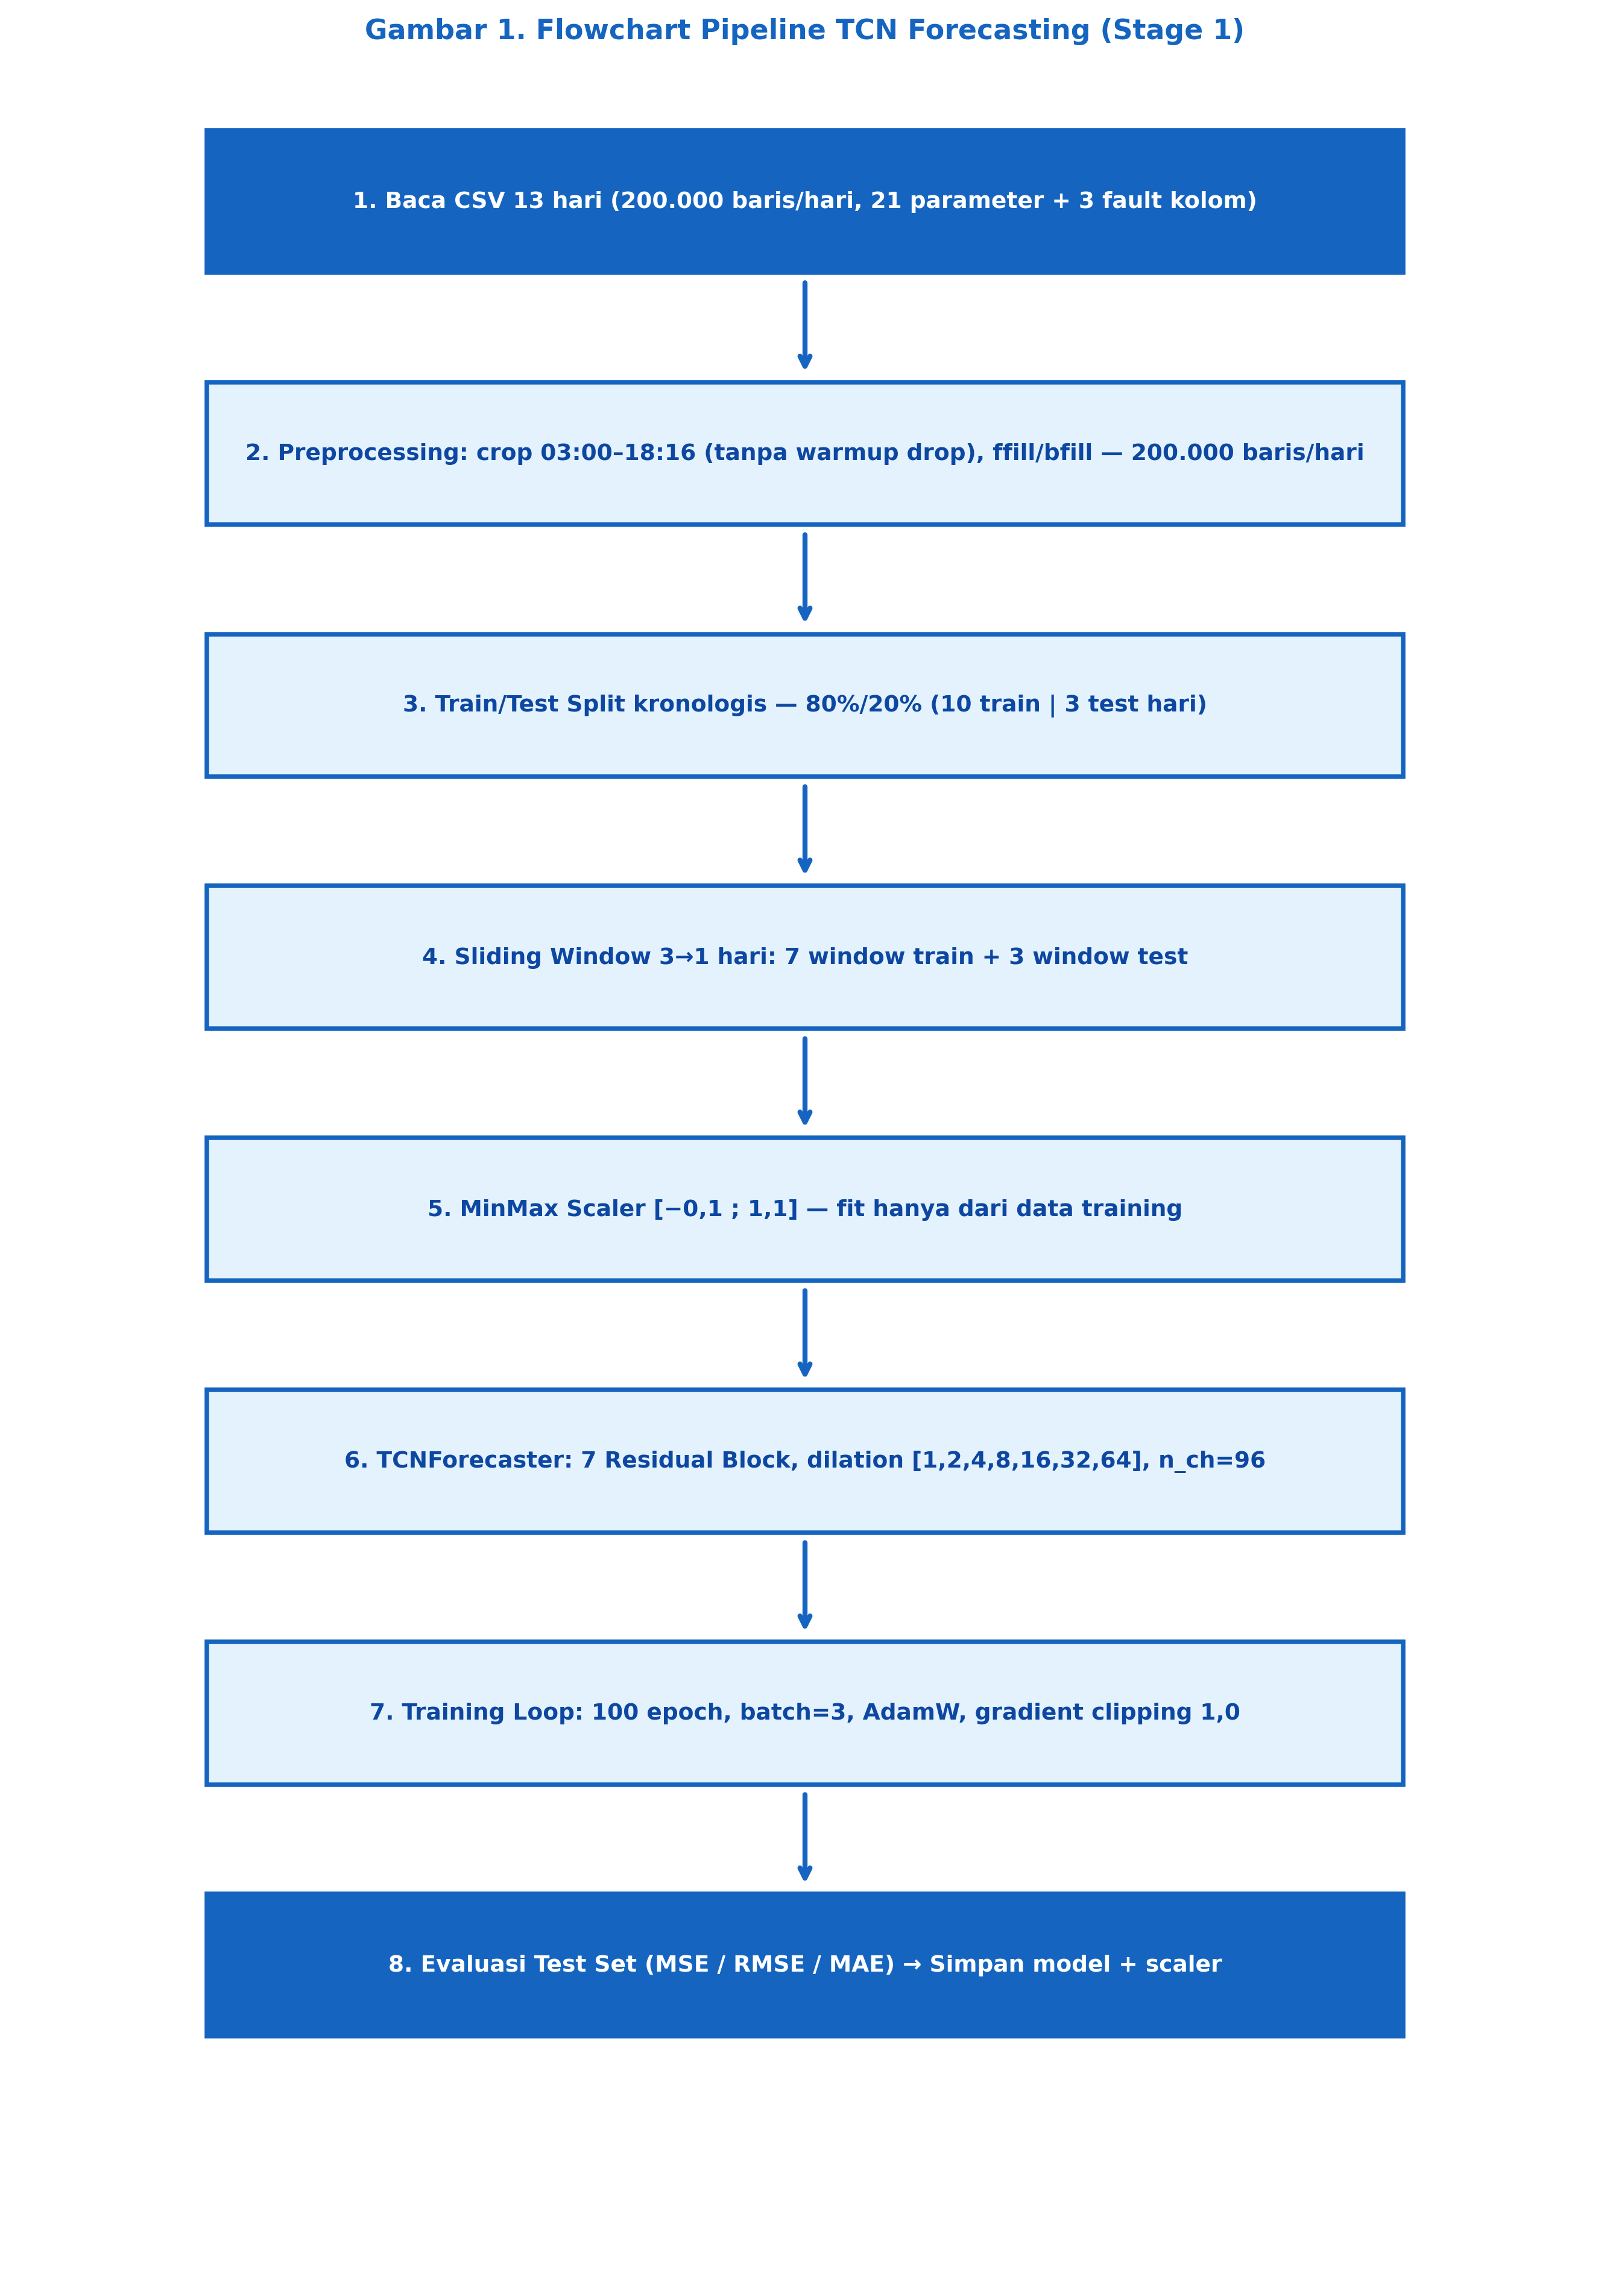
\includegraphics[width=0.95\linewidth]{jurnal_flowchart_stage1.png}
    \caption{Diagram alur (flowchart) pipeline Stage 1 — TCN Forecaster.}
    \label{fig:flow1}
\end{figure}

\begin{figure}[H]
    \centering
    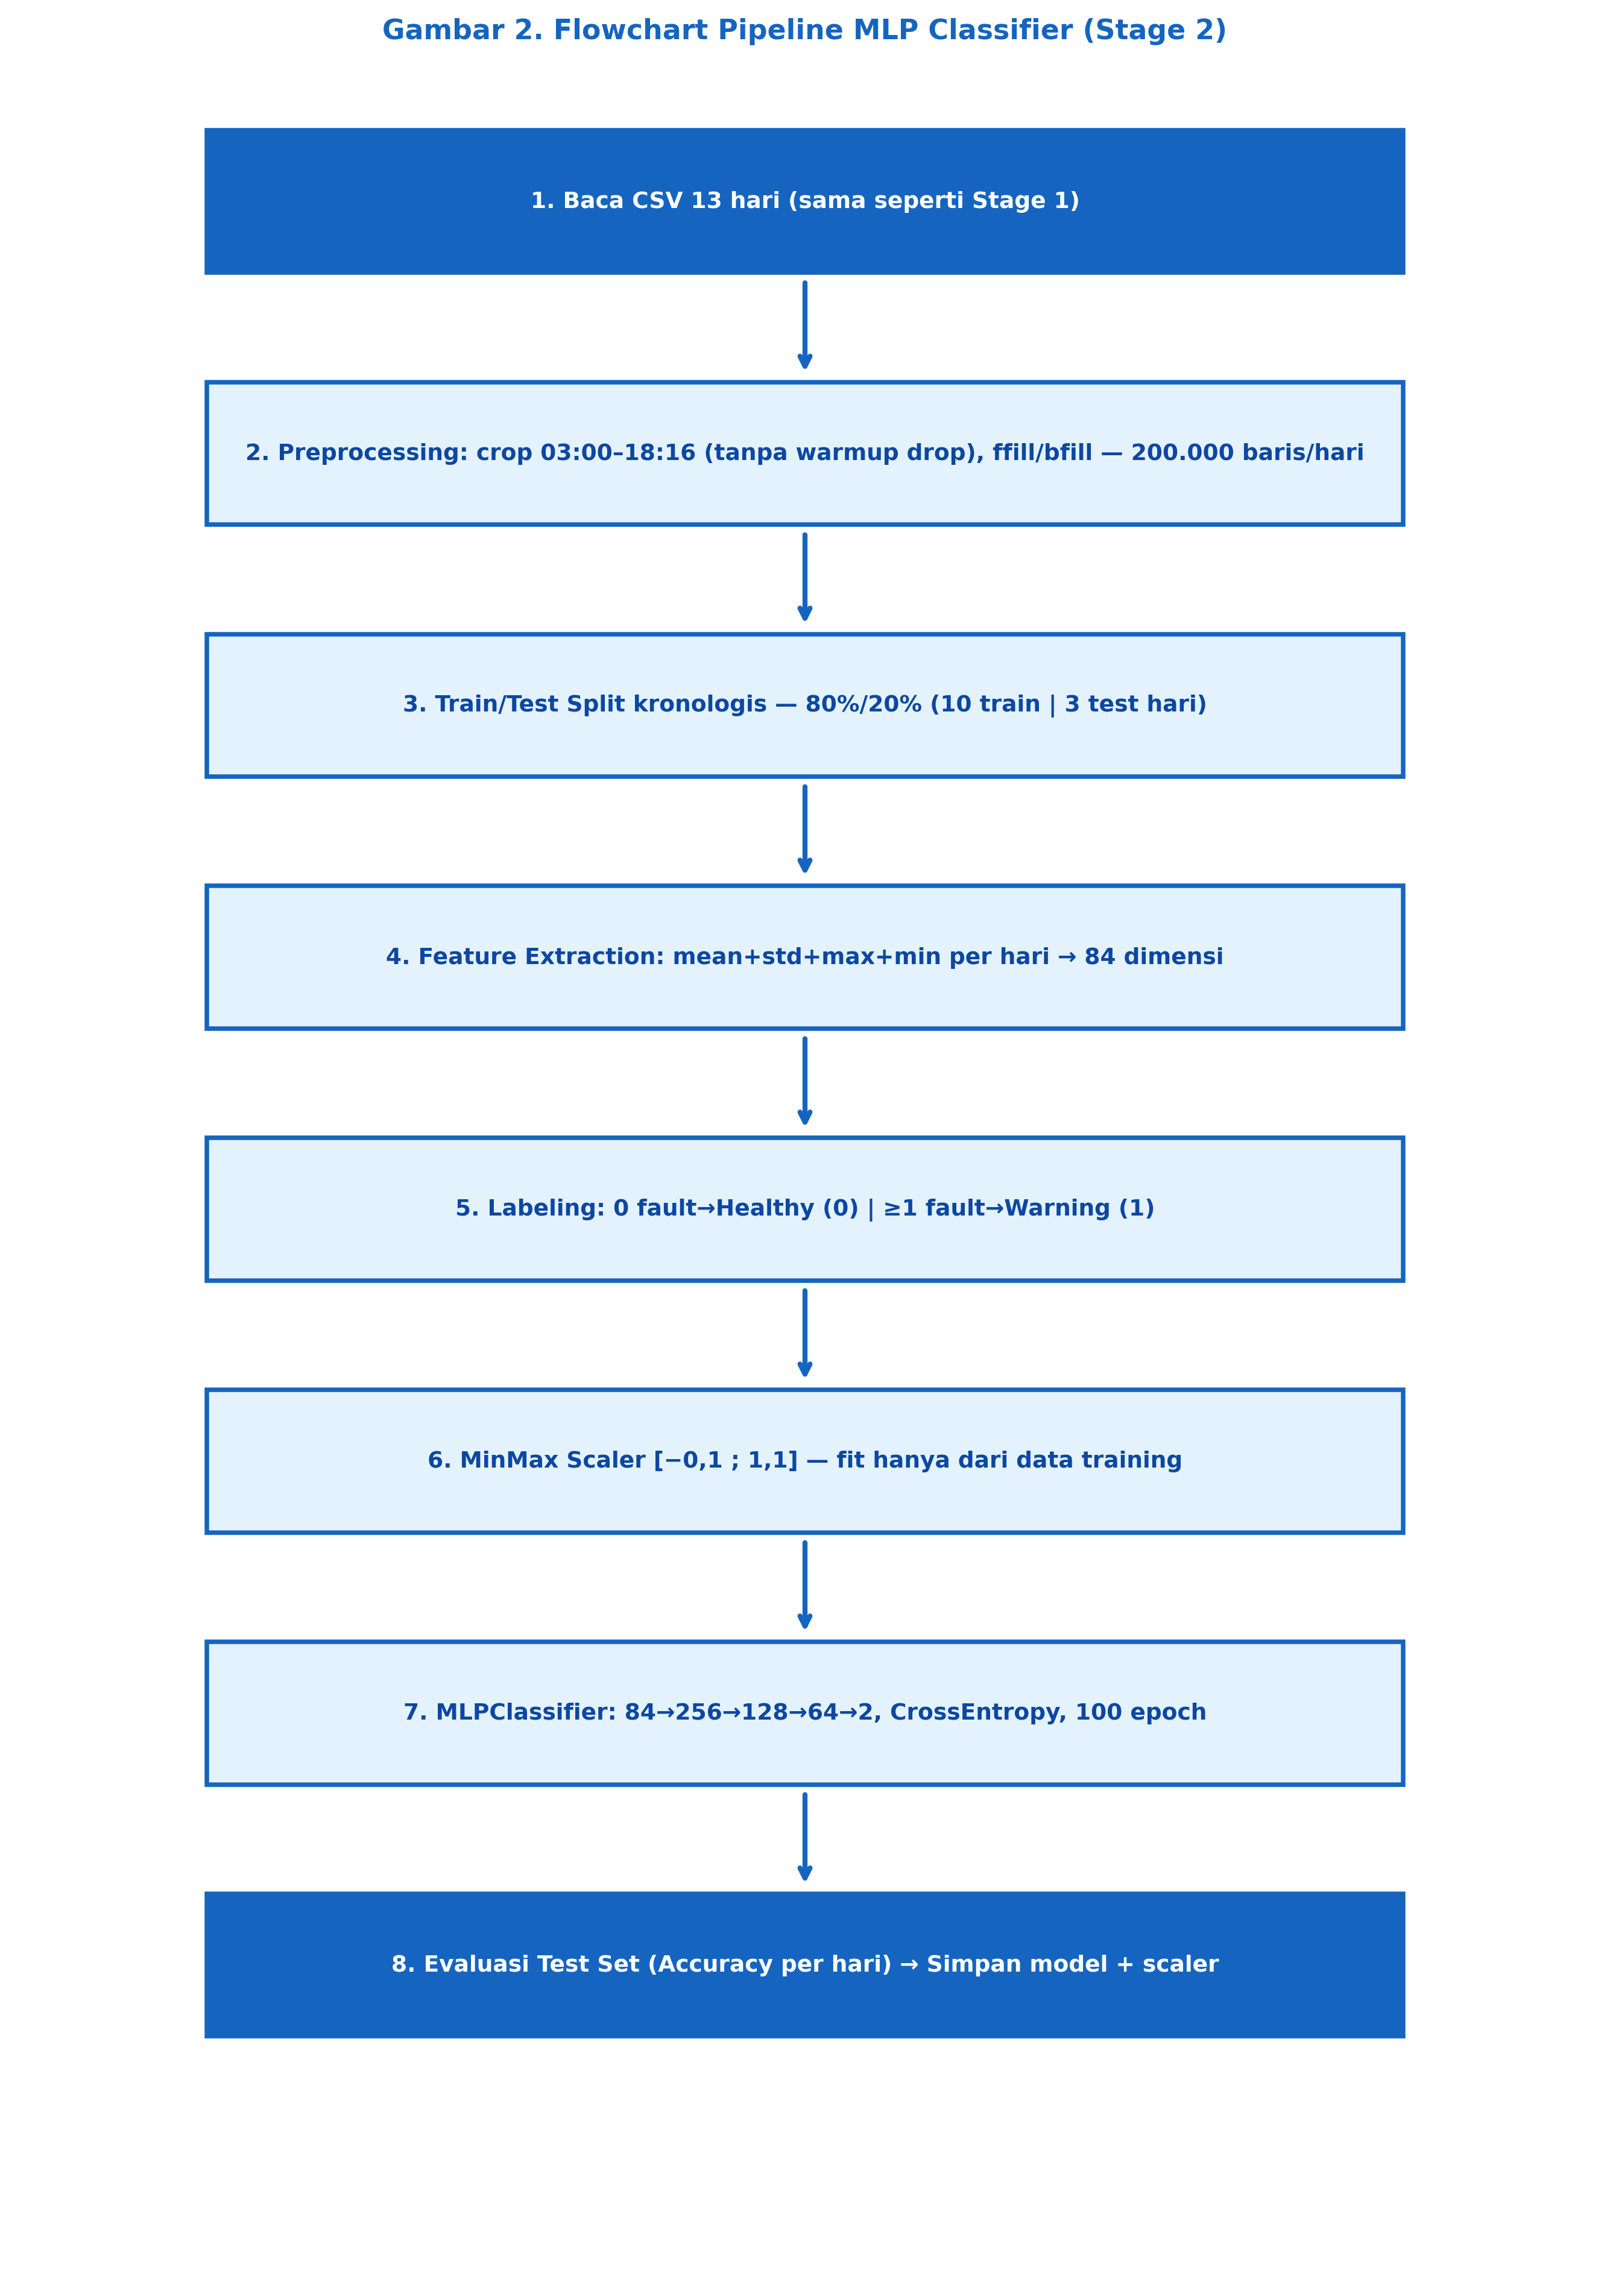
\includegraphics[width=0.95\linewidth]{jurnal_flowchart_stage2.png}
    \caption{Diagram alur (flowchart) pipeline Stage 2 — MLP Classifier.}
    \label{fig:flow2}
\end{figure}

\newpage
% ============================================================
\section{Dataset}
% ============================================================

\subsection{Ringkasan Umum}
\begin{table}[H]
    \centering
    \caption{Ringkasan dataset SIV TS27.}
    \begin{tabular}{ll}
        \toprule
        \textbf{Keterangan} & \textbf{Nilai} \\
        \midrule
        Total hari CSV valid & 37 hari \\
        Hari \textit{training} (80\%) & 29 hari \\
        Hari \textit{testing} (20\%) & 8 hari \\
        Baris per hari & 200.000 baris \\
        Total baris digunakan & 7.400.000 baris \\
        Jumlah parameter (fitur) & 21 parameter \\
        Window TCN (\textit{training}) & 26 window \\
        Window TCN (\textit{testing}) & 8 window (overlap 3 hari terakhir train) \\
        Missing value handling & forward-fill (ffill) + backward-fill (bfill) \\
        Rentang waktu harian & $\sim$03:00--03:27 WIB s/d 18:16 WIB \\
        \bottomrule
    \end{tabular}
\end{table}

Pembagian data mengikuti urutan waktu (\textit{chronological split}), bukan acak, sehingga tidak terjadi kebocoran data (\textit{data leakage}) dari masa depan ke masa lalu. Data \textit{training} mencakup Day 1--29 (02-01-2026 s/d 08-05-2026), sedangkan data \textit{testing} mencakup Day 30--37 (09-05-2026 s/d 23-05-2026).

\subsection{Detail Hari Training vs Testing}
\begin{longtable}{clcc}
    \toprule
    \textbf{Day} & \textbf{Tanggal} & \textbf{Set} & \textbf{Status Kesehatan} \\
    \midrule
    \endhead
    1  & 02012026 & Train & \warning \\
    2  & 10022026 & Train & \warning \\
    3  & 13022026 & Train & \healthy \\
    4  & 15022026 & Train & \healthy \\
    5  & 19022026 & Train & \healthy \\
    6  & 23022026 & Train & \healthy \\
    7  & 25022026 & Train & \healthy \\
    8  & 01032026 & Train & \warning \\
    9  & 07032026 & Train & \healthy \\
    10 & 22032026 & Train & \warning \\
    11 & 28032026 & Train & \healthy \\
    12 & 08042026 & Train & \healthy \\
    13 & 09042026 & Train & \healthy \\
    14 & 11042026 & Train & \healthy \\
    15 & 12042026 & Train & \healthy \\
    16 & 15042026 & Train & \healthy \\
    17 & 16042026 & Train & \healthy \\
    18 & 17042026 & Train & \healthy \\
    19 & 19042026 & Train & \healthy \\
    20 & 21042026 & Train & \warning \\
    21 & 22042026 & Train & \healthy \\
    22 & 23042026 & Train & \warning \\
    23 & 24042026 & Train & \healthy \\
    24 & 27042026 & Train & \warning \\
    25 & 04052026 & Train & \healthy \\
    26 & 05052026 & Train & \warning \\
    27 & 06052026 & Train & \warning \\
    28 & 07052026 & Train & \healthy \\
    29 & 08052026 & Train & \healthy \\
    30 & 09052026 & Test  & \healthy \\
    31 & 14052026 & Test  & \warning \\
    32 & 15052026 & Test  & \healthy \\
    33 & 16052026 & Test  & \healthy \\
    34 & 17052026 & Test  & \healthy \\
    35 & 20052026 & Test  & \warning \\
    36 & 22052026 & Test  & \warning \\
    37 & 23052026 & Test  & \healthy \\
    \bottomrule
    \caption{Detail 37 hari data beserta pembagian set dan status kesehatan aktual.}
    \label{tab:days}
\end{longtable}

\textbf{Distribusi label keseluruhan (37 hari):} 25 hari \healthy\ (67.6\%), 12 hari \warning\ (32.4\%).

\newpage
\subsection{Visualisasi Seluruh Parameter}
\begin{figure}[H]
    \centering
    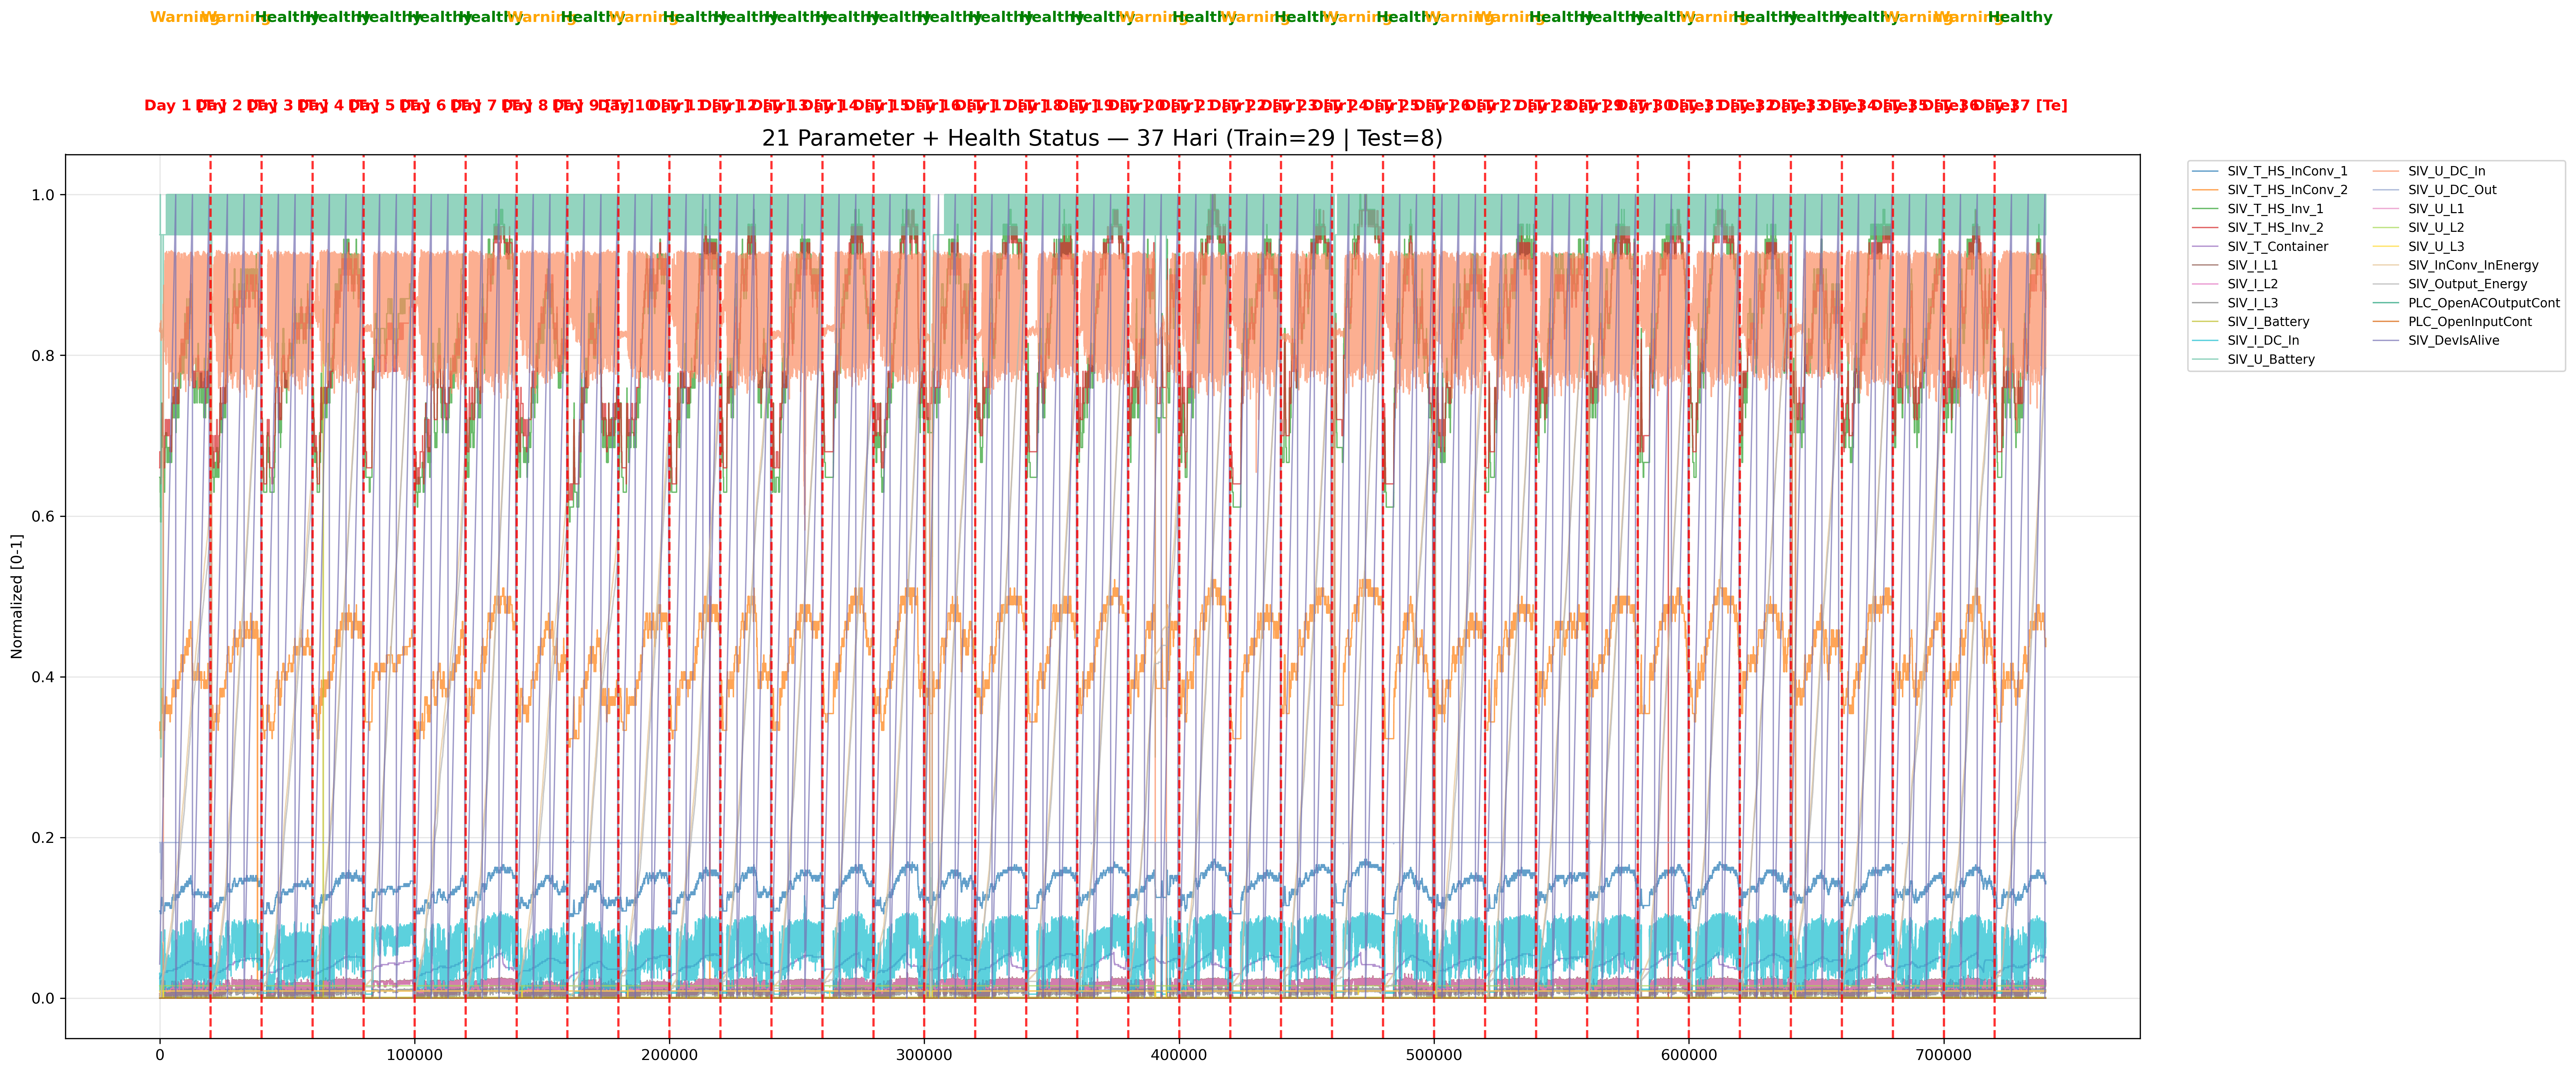
\includegraphics[width=\linewidth]{plot_all_parameters_TCN.png}
    \caption{Plot 21 parameter sensor untuk seluruh hari dataset (supplementary).}
    \label{fig:allparam}
\end{figure}

\newpage
% ============================================================
\section{Preprocessing dan Normalisasi}
% ============================================================

\subsection{Normalisasi Min-Max}
Seluruh 21 parameter dinormalisasi menggunakan \textbf{Min-Max Scaler} ke rentang $[-0.1,\ 1.1]$. Scaler di-\textit{fit} hanya pada 29 hari data \textit{training} untuk mencegah kebocoran data, kemudian diterapkan (\textit{transform}) pada data \textit{training} maupun \textit{testing}.

\begin{longtable}{lrr}
    \toprule
    \textbf{Parameter} & \textbf{Min Data} & \textbf{Max Data} \\
    \midrule
    \endhead
    SIV\_T\_HS\_InConv\_1   & 0.0000   & 295.0000 \\
    SIV\_T\_HS\_InConv\_2   & 0.0000   & 96.0000 \\
    SIV\_T\_HS\_Inv\_1      & 31.0000  & 54.0000 \\
    SIV\_T\_HS\_Inv\_2      & 31.0000  & 50.0000 \\
    SIV\_T\_Container       & 30.0000  & 557.0000 \\
    SIV\_I\_L1              & 0.0000   & 4144.0000 \\
    SIV\_I\_L2              & 0.0000   & 126.0000 \\
    SIV\_I\_L3              & 0.0000   & 8198.0000 \\
    SIV\_I\_Battery         & -33.0000 & 24800.0000 \\
    SIV\_I\_DC\_In          & 0.0000   & 544.0000 \\
    SIV\_U\_Battery         & 94.0000  & 114.0000 \\
    SIV\_U\_DC\_In          & 0.0000   & 936.0000 \\
    SIV\_U\_DC\_Out         & 3.0000   & 127.0000 \\
    SIV\_U\_L1              & 0.0000   & 24768.0000 \\
    SIV\_U\_L2              & 0.0000   & 14272.0000 \\
    SIV\_U\_L3              & 0.0000   & 24603.0000 \\
    SIV\_InConv\_InEnergy   & 0.0000   & 644.0000 \\
    SIV\_Output\_Energy     & 0.0000   & 574.0000 \\
    PLC\_OpenACOutputCont   & 0.0000   & 0.0000 \\
    PLC\_OpenInputCont      & 0.0000   & 0.0000 \\
    SIV\_DevIsAlive         & 0.0000   & 65535.0000 \\
    \bottomrule
    \caption{Rentang nilai (min--max) 21 parameter dari scaler training.}
    \label{tab:minmax}
\end{longtable}

\begin{figure}[H]
    \centering
    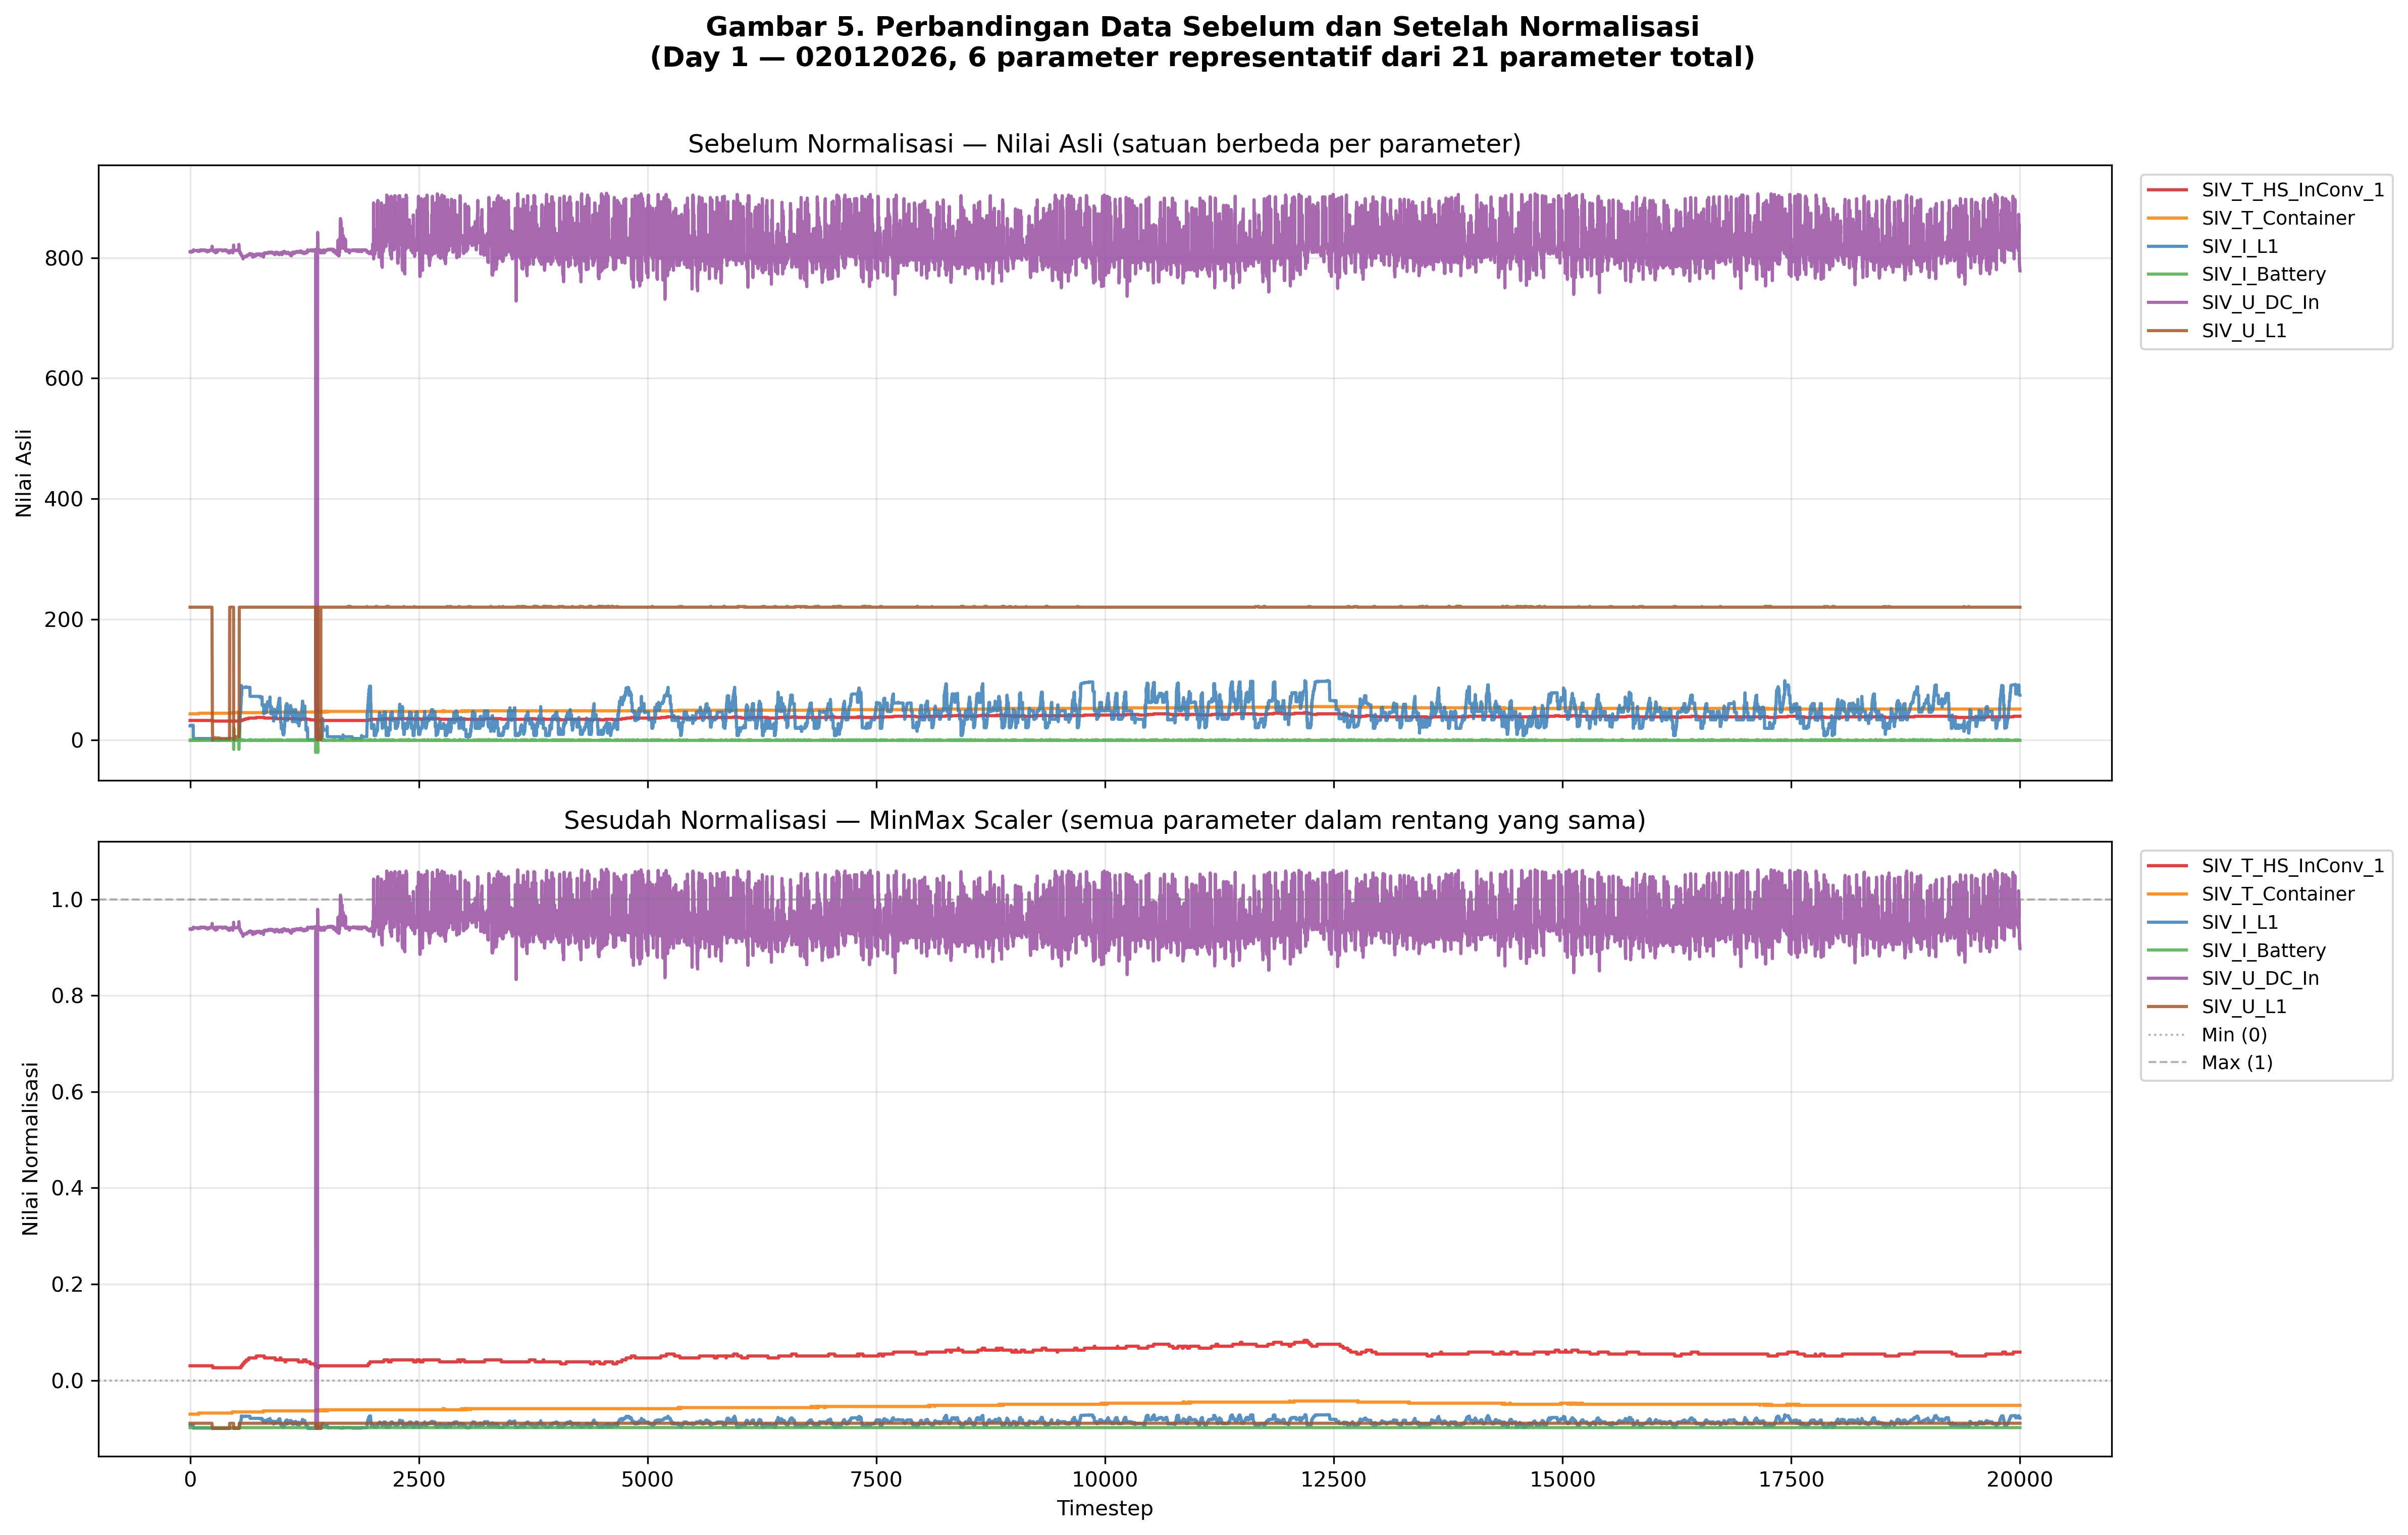
\includegraphics[width=0.9\linewidth]{jurnal_normalisasi_comparison.png}
    \caption{Perbandingan data sebelum vs sesudah normalisasi Min-Max.}
    \label{fig:norm}
\end{figure}

\subsection{Skema Sliding Window}
Sequence input-output dibentuk menggunakan skema \textit{sliding window} 3 hari input $\rightarrow$ 1 hari target (H+1), digeser satu hari setiap langkah.

\begin{figure}[H]
    \centering
    \includegraphics[width=0.85\linewidth]{jurnal_sliding_window.png}
    \caption{Skema sliding window: 3 hari input memprediksi 1 hari target berikutnya.}
    \label{fig:slidewin}
\end{figure}

\newpage
% ============================================================
\section{Stage 1 — TCN Forecaster}
% ============================================================

\subsection{Arsitektur}
\begin{table}[H]
    \centering
    \caption{Arsitektur TCN (Temporal Convolutional Network).}
    \begin{tabular}{ll}
        \toprule
        \textbf{Komponen} & \textbf{Spesifikasi} \\
        \midrule
        Jumlah Residual Block & 7 \\
        Dilation Factors & [1, 2, 4, 8, 16, 32, 64] \\
        Hidden Channel ($n_{ch}$) & 96 \\
        Kernel Size & 3 \\
        Input Window & 3 hari = 600.000 timestep \\
        Output Horizon & H+1 = 200.000 timestep (1 hari) \\
        Input Shape & (batch, 600000, 21) \\
        Output Shape & (batch, 200000, 21) \\
        \bottomrule
    \end{tabular}
\end{table}

\subsection{Hyperparameter Training}
\begin{table}[H]
    \centering
    \caption{Hyperparameter training Stage 1 (TCN Forecaster).}
    \begin{tabular}{ll}
        \toprule
        \textbf{Hyperparameter} & \textbf{Nilai} \\
        \midrule
        Optimizer & AdamW \\
        Learning Rate (awal) & 0.001 \\
        Learning Rate (akhir) & 1.00e-03 \\
        Batch Size & 3 \\
        Epoch & 100 \\
        Loss Function & Mean Squared Error (MSE) \\
        Gradient Clipping & 1.0 \\
        Dropout & 0.3 \\
        Weight Decay & 1e-5 \\
        Scheduler & ReduceLROnPlateau (factor=0.5, patience=30) \\
        \bottomrule
    \end{tabular}
\end{table}

\subsection{Hasil Training}
Loss (MSE) menurun dari \textbf{0.3568467} (35.68\%) pada epoch 1 menjadi \textbf{0.0120068} (1.20\%) pada epoch 100, atau penurunan total sebesar \textbf{96.6\%}.

\begin{figure}[H]
    \centering
    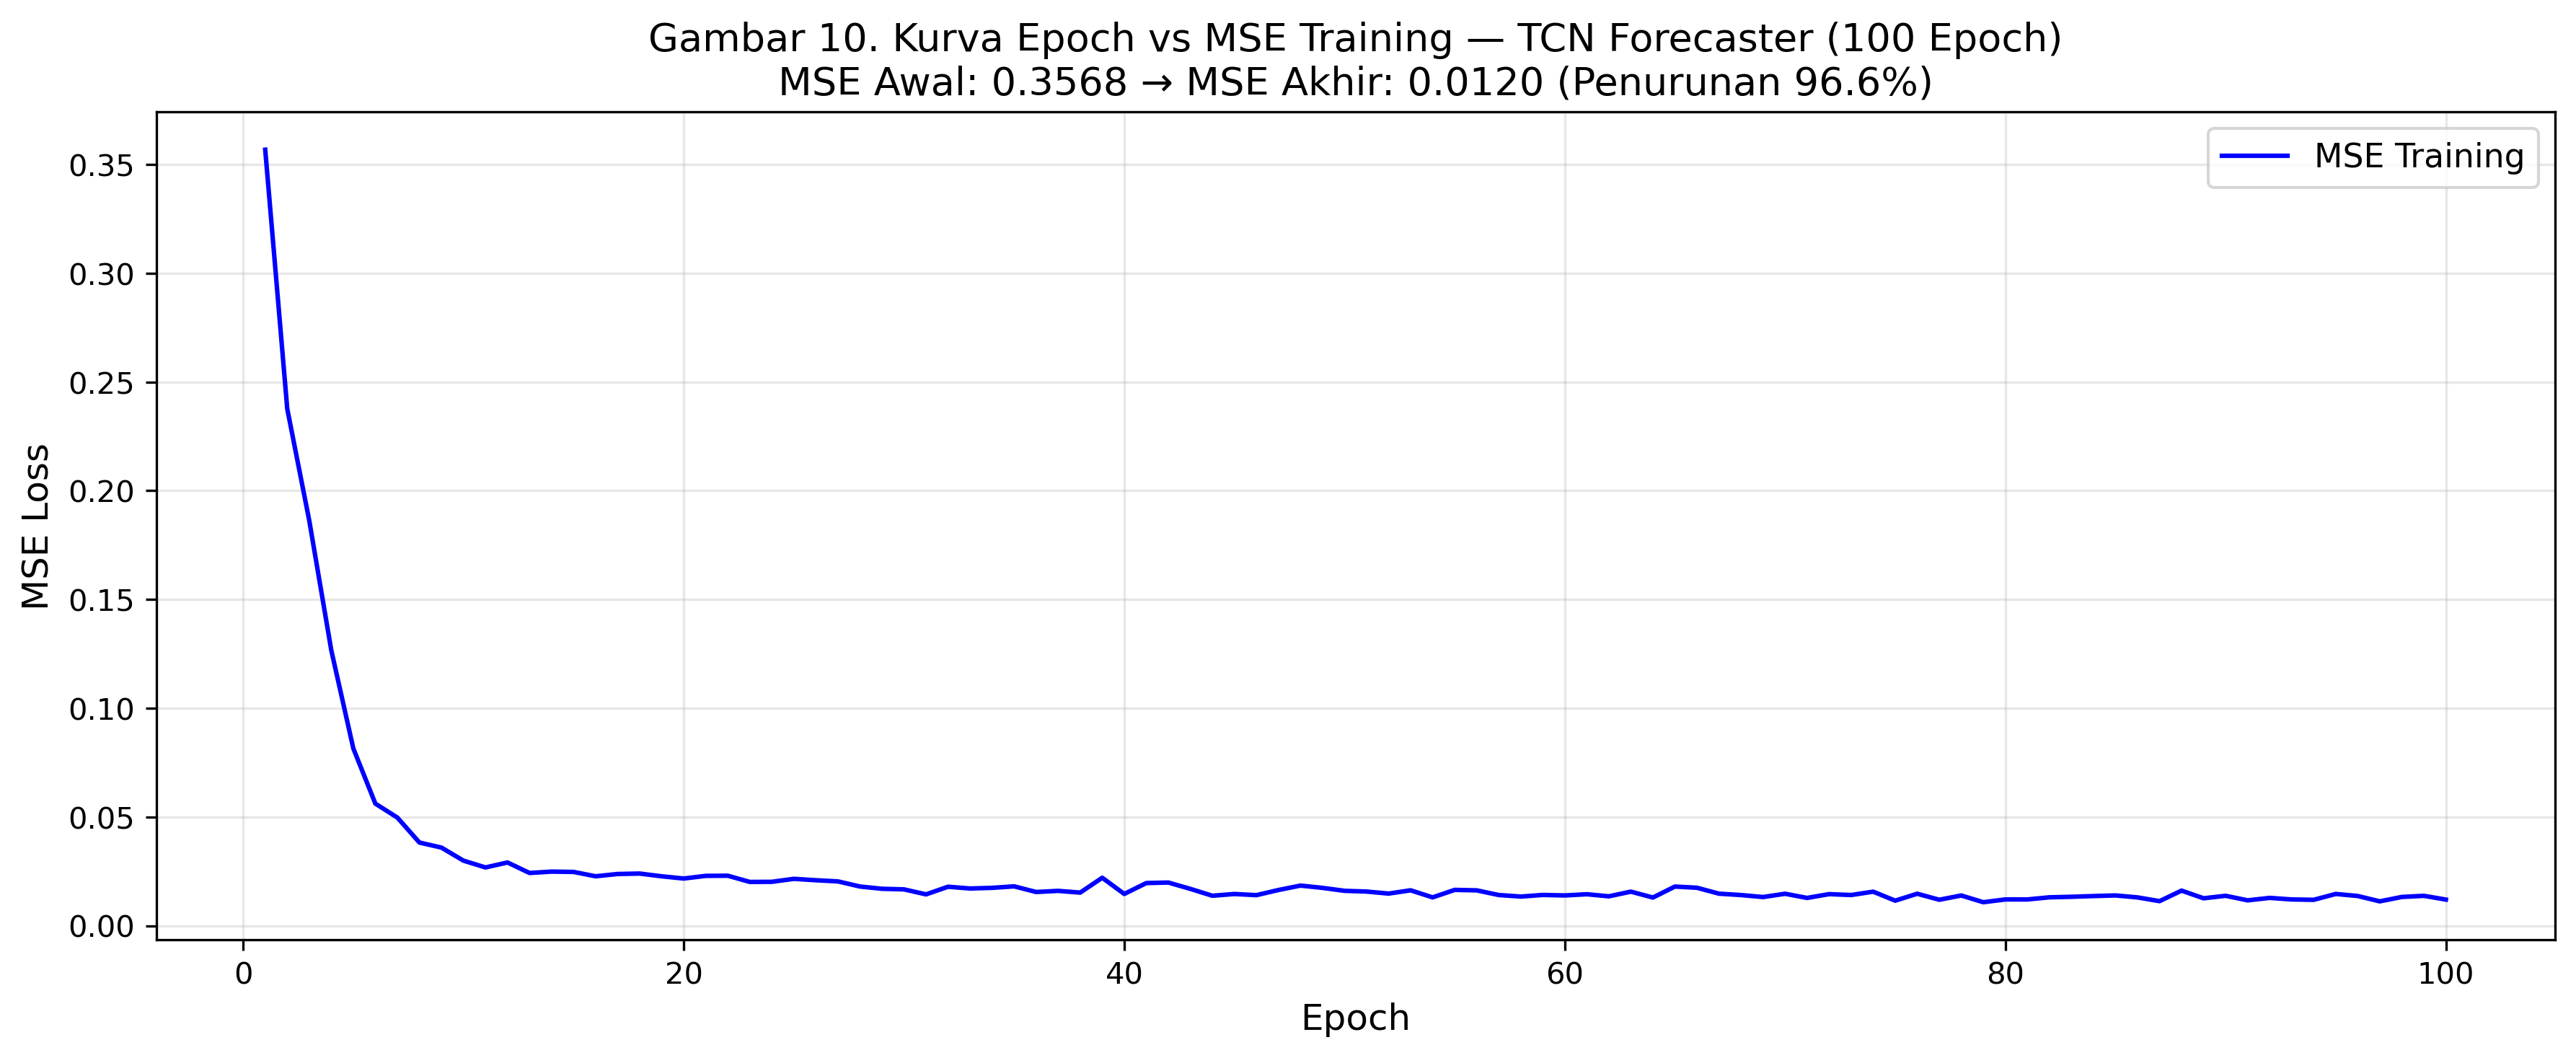
\includegraphics[width=0.85\linewidth]{jurnal_kurva_loss_stage1.png}
    \caption{Kurva Epoch vs MSE selama training Stage 1 (TCN Forecaster).}
    \label{fig:loss1}
\end{figure}

\subsection{Evaluasi Training vs Testing}
\begin{table}[H]
    \centering
    \caption{Metrik evaluasi Stage 1 pada skala ternormalisasi $[-0.1, 1.1]$.}
    \begin{tabular}{lrr}
        \toprule
        \textbf{Metrik} & \textbf{Training Set (26 window)} & \textbf{Test Set (8 window)} \\
        \midrule
        MSE  & 0.008066 & 0.007446 \\
        RMSE & 0.089810 & 0.086292 \\
        MAE  & 0.046303 & 0.043340 \\
        MAPE & 44.83\%  & 42.43\% \\
        \bottomrule
    \end{tabular}
\end{table}

\noindent\textbf{Catatan:} Selisih MSE train--test sangat kecil (0.00456), mengindikasikan model TCN \textbf{tidak overfitting} dan generalisasi dengan baik terhadap data yang belum pernah dilihat.

\subsection{Pembentukan Sequence (Sliding Window Detail)}
\begin{longtable}{clllll}
    \toprule
    \textbf{Seq} & \textbf{Input A} & \textbf{Input B} & \textbf{Input C} & \textbf{Target H+1} & \textbf{Set} \\
    \midrule
    \endhead
    1  & 02012026 & 10022026 & 13022026 & 15022026 & Training \\
    2  & 10022026 & 13022026 & 15022026 & 19022026 & Training \\
    3  & 13022026 & 15022026 & 19022026 & 23022026 & Training \\
    4  & 15022026 & 19022026 & 23022026 & 25022026 & Training \\
    5  & 19022026 & 23022026 & 25022026 & 01032026 & Training \\
    6  & 23022026 & 25022026 & 01032026 & 07032026 & Training \\
    7  & 25022026 & 01032026 & 07032026 & 22032026 & Training \\
    8  & 01032026 & 07032026 & 22032026 & 28032026 & Training \\
    9  & 07032026 & 22032026 & 28032026 & 08042026 & Training \\
    10 & 22032026 & 28032026 & 08042026 & 09042026 & Training \\
    11 & 28032026 & 08042026 & 09042026 & 11042026 & Training \\
    12 & 08042026 & 09042026 & 11042026 & 12042026 & Training \\
    13 & 09042026 & 11042026 & 12042026 & 15042026 & Training \\
    14 & 11042026 & 12042026 & 15042026 & 16042026 & Training \\
    15 & 12042026 & 15042026 & 16042026 & 17042026 & Training \\
    16 & 15042026 & 16042026 & 17042026 & 19042026 & Training \\
    17 & 16042026 & 17042026 & 19042026 & 21042026 & Training \\
    18 & 17042026 & 19042026 & 21042026 & 22042026 & Training \\
    19 & 19042026 & 21042026 & 22042026 & 23042026 & Training \\
    20 & 21042026 & 22042026 & 23042026 & 24042026 & Training \\
    21 & 22042026 & 23042026 & 24042026 & 27042026 & Training \\
    22 & 23042026 & 24042026 & 27042026 & 04052026 & Training \\
    23 & 24042026 & 27042026 & 04052026 & 05052026 & Training \\
    24 & 27042026 & 04052026 & 05052026 & 06052026 & Training \\
    25 & 04052026 & 05052026 & 06052026 & 07052026 & Training \\
    26 & 05052026 & 06052026 & 07052026 & 08052026 & Training \\
    27 & 06052026 & 07052026 & 08052026 & 09052026 & Testing \\
    28 & 07052026 & 08052026 & 09052026 & 14052026 & Testing \\
    29 & 08052026 & 09052026 & 14052026 & 15052026 & Testing \\
    30 & 09052026 & 14052026 & 15052026 & 16052026 & Testing \\
    31 & 14052026 & 15052026 & 16052026 & 17052026 & Testing \\
    32 & 15052026 & 16052026 & 17052026 & 20052026 & Testing \\
    33 & 16052026 & 17052026 & 20052026 & 22052026 & Testing \\
    34 & 17052026 & 20052026 & 22052026 & 23052026 & Testing \\
    \bottomrule
    \caption{Detail pembentukan 34 sequence sliding-window (3 hari input $\to$ 1 hari target).}
    \label{tab:seq}
\end{longtable}

\newpage
% ============================================================
\section{Stage 2 — MLP Classifier}
% ============================================================

\subsection{Ekstraksi Fitur}
Hasil forecast Stage 1 (200.000 timestep $\times$ 21 parameter) diringkas menjadi \textbf{84 fitur statistik} (mean, std, min, max $\times$ 21 parameter) sebagai input MLP Classifier.

\subsection{Arsitektur}
\begin{table}[H]
    \centering
    \caption{Arsitektur MLP Classifier.}
    \begin{tabular}{ll}
        \toprule
        \textbf{Layer} & \textbf{Spesifikasi} \\
        \midrule
        Input Layer   & 84 neuron (84 fitur statistik) \\
        Hidden Layer 1 & 256 neuron + LayerNorm + ReLU + Dropout \\
        Hidden Layer 2 & 128 neuron + LayerNorm + ReLU + Dropout \\
        Hidden Layer 3 & 64 neuron + LayerNorm + ReLU + Dropout \\
        Output Layer  & 2 neuron (Softmax) — Healthy / Warning \\
        \bottomrule
    \end{tabular}
\end{table}

\subsection{Hyperparameter Training}
\begin{table}[H]
    \centering
    \caption{Hyperparameter training Stage 2 (MLP Classifier).}
    \begin{tabular}{ll}
        \toprule
        \textbf{Hyperparameter} & \textbf{Nilai} \\
        \midrule
        Optimizer & AdamW \\
        Learning Rate (awal) & 0.001 \\
        Batch Size & 3 \\
        Epoch & 100 \\
        Loss Function & Cross-Entropy Loss \\
        Class Weight & Healthy = 0.5, Warning = 2.5 \\
        Dropout & 0.3 \\
        Weight Decay & 1e-5 \\
        Scheduler & ReduceLROnPlateau (factor=0.5, patience=30) \\
        \bottomrule
    \end{tabular}
\end{table}

\subsection{Distribusi Label}
\begin{table}[H]
    \centering
    \caption{Distribusi label 37 hari.}
    \begin{tabular}{lrl}
        \toprule
        \textbf{Kelas} & \textbf{Jumlah Hari} & \textbf{Set} \\
        \midrule
        \healthy\ (0) & 25 hari (20 train / 5 test) & Train + Test \\
        \warning\ (1) & 12 hari (9 train / 3 test)  & Train + Test \\
        \bottomrule
    \end{tabular}
\end{table}

\subsection{Hasil Training}
CE Loss menurun dari \textbf{1.005112} (epoch 1) menjadi \textbf{0.068207} (epoch 100) — penurunan \textbf{93.2\%}. Akurasi training meningkat dari 66.67\% menjadi 96.30\%, bahkan mencapai 100\% pada banyak epoch di paruh kedua training.

\begin{figure}[H]
    \centering
    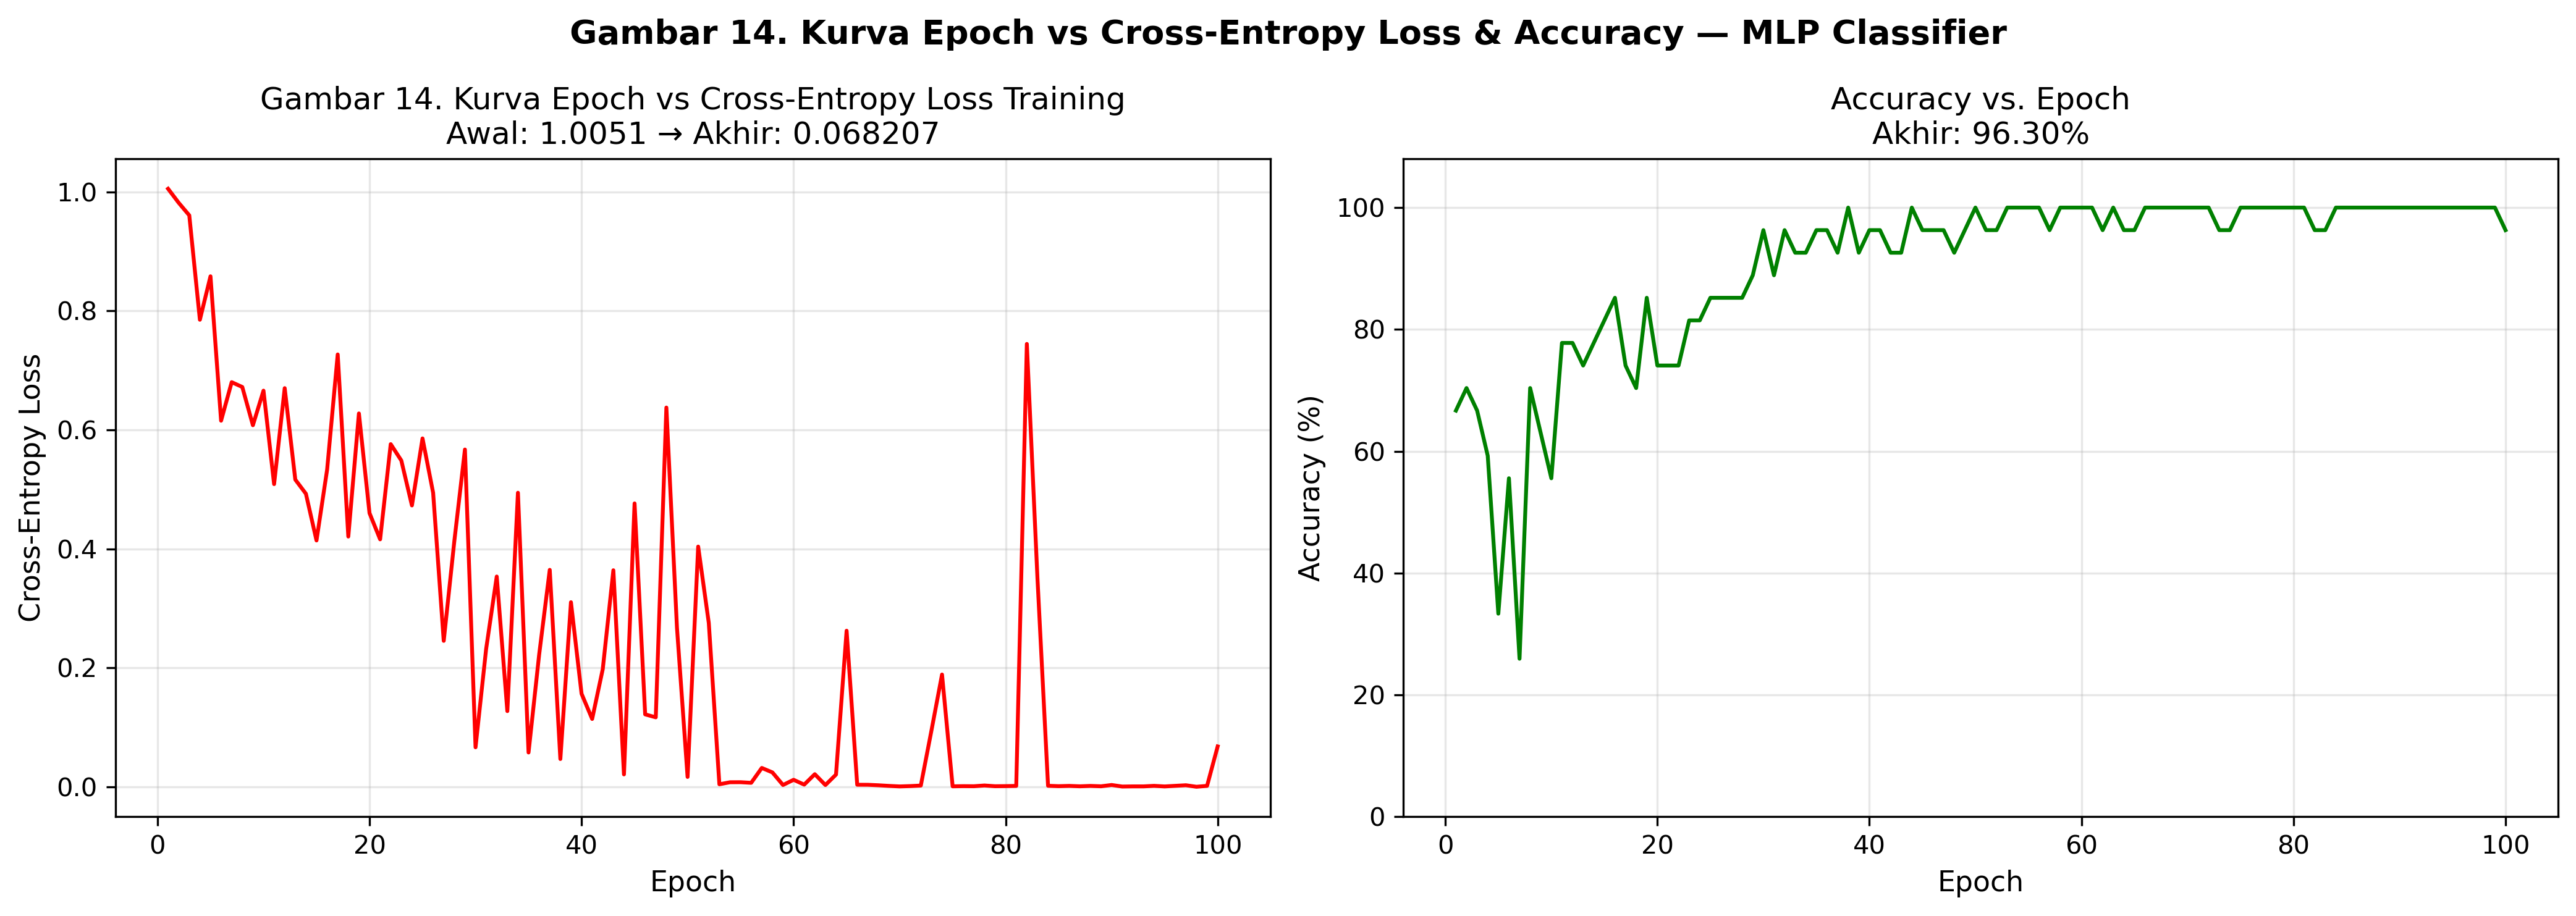
\includegraphics[width=0.85\linewidth]{jurnal_kurva_loss_acc_stage2.png}
    \caption{Kurva CE Loss dan Accuracy selama training Stage 2 (MLP Classifier).}
    \label{fig:loss2}
\end{figure}

\subsection{Evaluasi Training Set}
\begin{table}[H]
    \centering
    \caption{Metrik evaluasi Stage 2 — Training Set (29 hari).}
    \begin{tabular}{lr}
        \toprule
        \textbf{Metrik} & \textbf{Nilai} \\
        \midrule
        CE Loss   & 0.000223 \\
        Accuracy  & 100.00\% \\
        Precision & 100.00\% \\
        Recall    & 100.00\% \\
        F1-Score  & 100.00\% \\
        \bottomrule
    \end{tabular}
\end{table}

\begin{table}[H]
    \centering
    \caption{Confusion matrix — Training Set.}
    \begin{tabular}{lcc}
        \toprule
         & \textbf{Pred Healthy} & \textbf{Pred Warning} \\
        \midrule
        \textbf{Aktual Healthy} & 20 & 0 \\
        \textbf{Aktual Warning} & 0  & 9 \\
        \bottomrule
    \end{tabular}
\end{table}

\subsection{Evaluasi Test Set}
\begin{table}[H]
    \centering
    \caption{Metrik evaluasi Stage 2 — Test Set (8 hari).}
    \begin{tabular}{lr}
        \toprule
        \textbf{Metrik} & \textbf{Nilai} \\
        \midrule
        CE Loss   & 5.903700 \\
        Accuracy  & 62.50\% \\
        Precision & 39.06\% \\
        Recall    & 62.50\% \\
        F1-Score  & 48.08\% \\
        \bottomrule
    \end{tabular}
\end{table}

\begin{table}[H]
    \centering
    \caption{Confusion matrix — Test Set.}
    \begin{tabular}{lcc}
        \toprule
         & \textbf{Pred Healthy} & \textbf{Pred Warning} \\
        \midrule
        \textbf{Aktual Healthy} & 5 & 0 \\
        \textbf{Aktual Warning} & 3 & 0 \\
        \bottomrule
    \end{tabular}
\end{table}

\begin{table}[H]
    \centering
    \caption{Detail prediksi per hari — Test Set.}
    \begin{tabular}{clllc}
        \toprule
        \textbf{Day} & \textbf{Tanggal} & \textbf{Aktual} & \textbf{Prediksi} & \textbf{Benar?} \\
        \midrule
        30 & 09052026 & \healthy & \healthy & \ok \\
        31 & 14052026 & \warning & \healthy & \bad \\
        32 & 15052026 & \healthy & \healthy & \ok \\
        33 & 16052026 & \healthy & \healthy & \ok \\
        34 & 17052026 & \healthy & \healthy & \ok \\
        35 & 20052026 & \warning & \healthy & \bad \\
        36 & 22052026 & \warning & \healthy & \bad \\
        37 & 23052026 & \healthy & \healthy & \ok \\
        \bottomrule
    \end{tabular}
\end{table}

\begin{figure}[H]
    \centering
    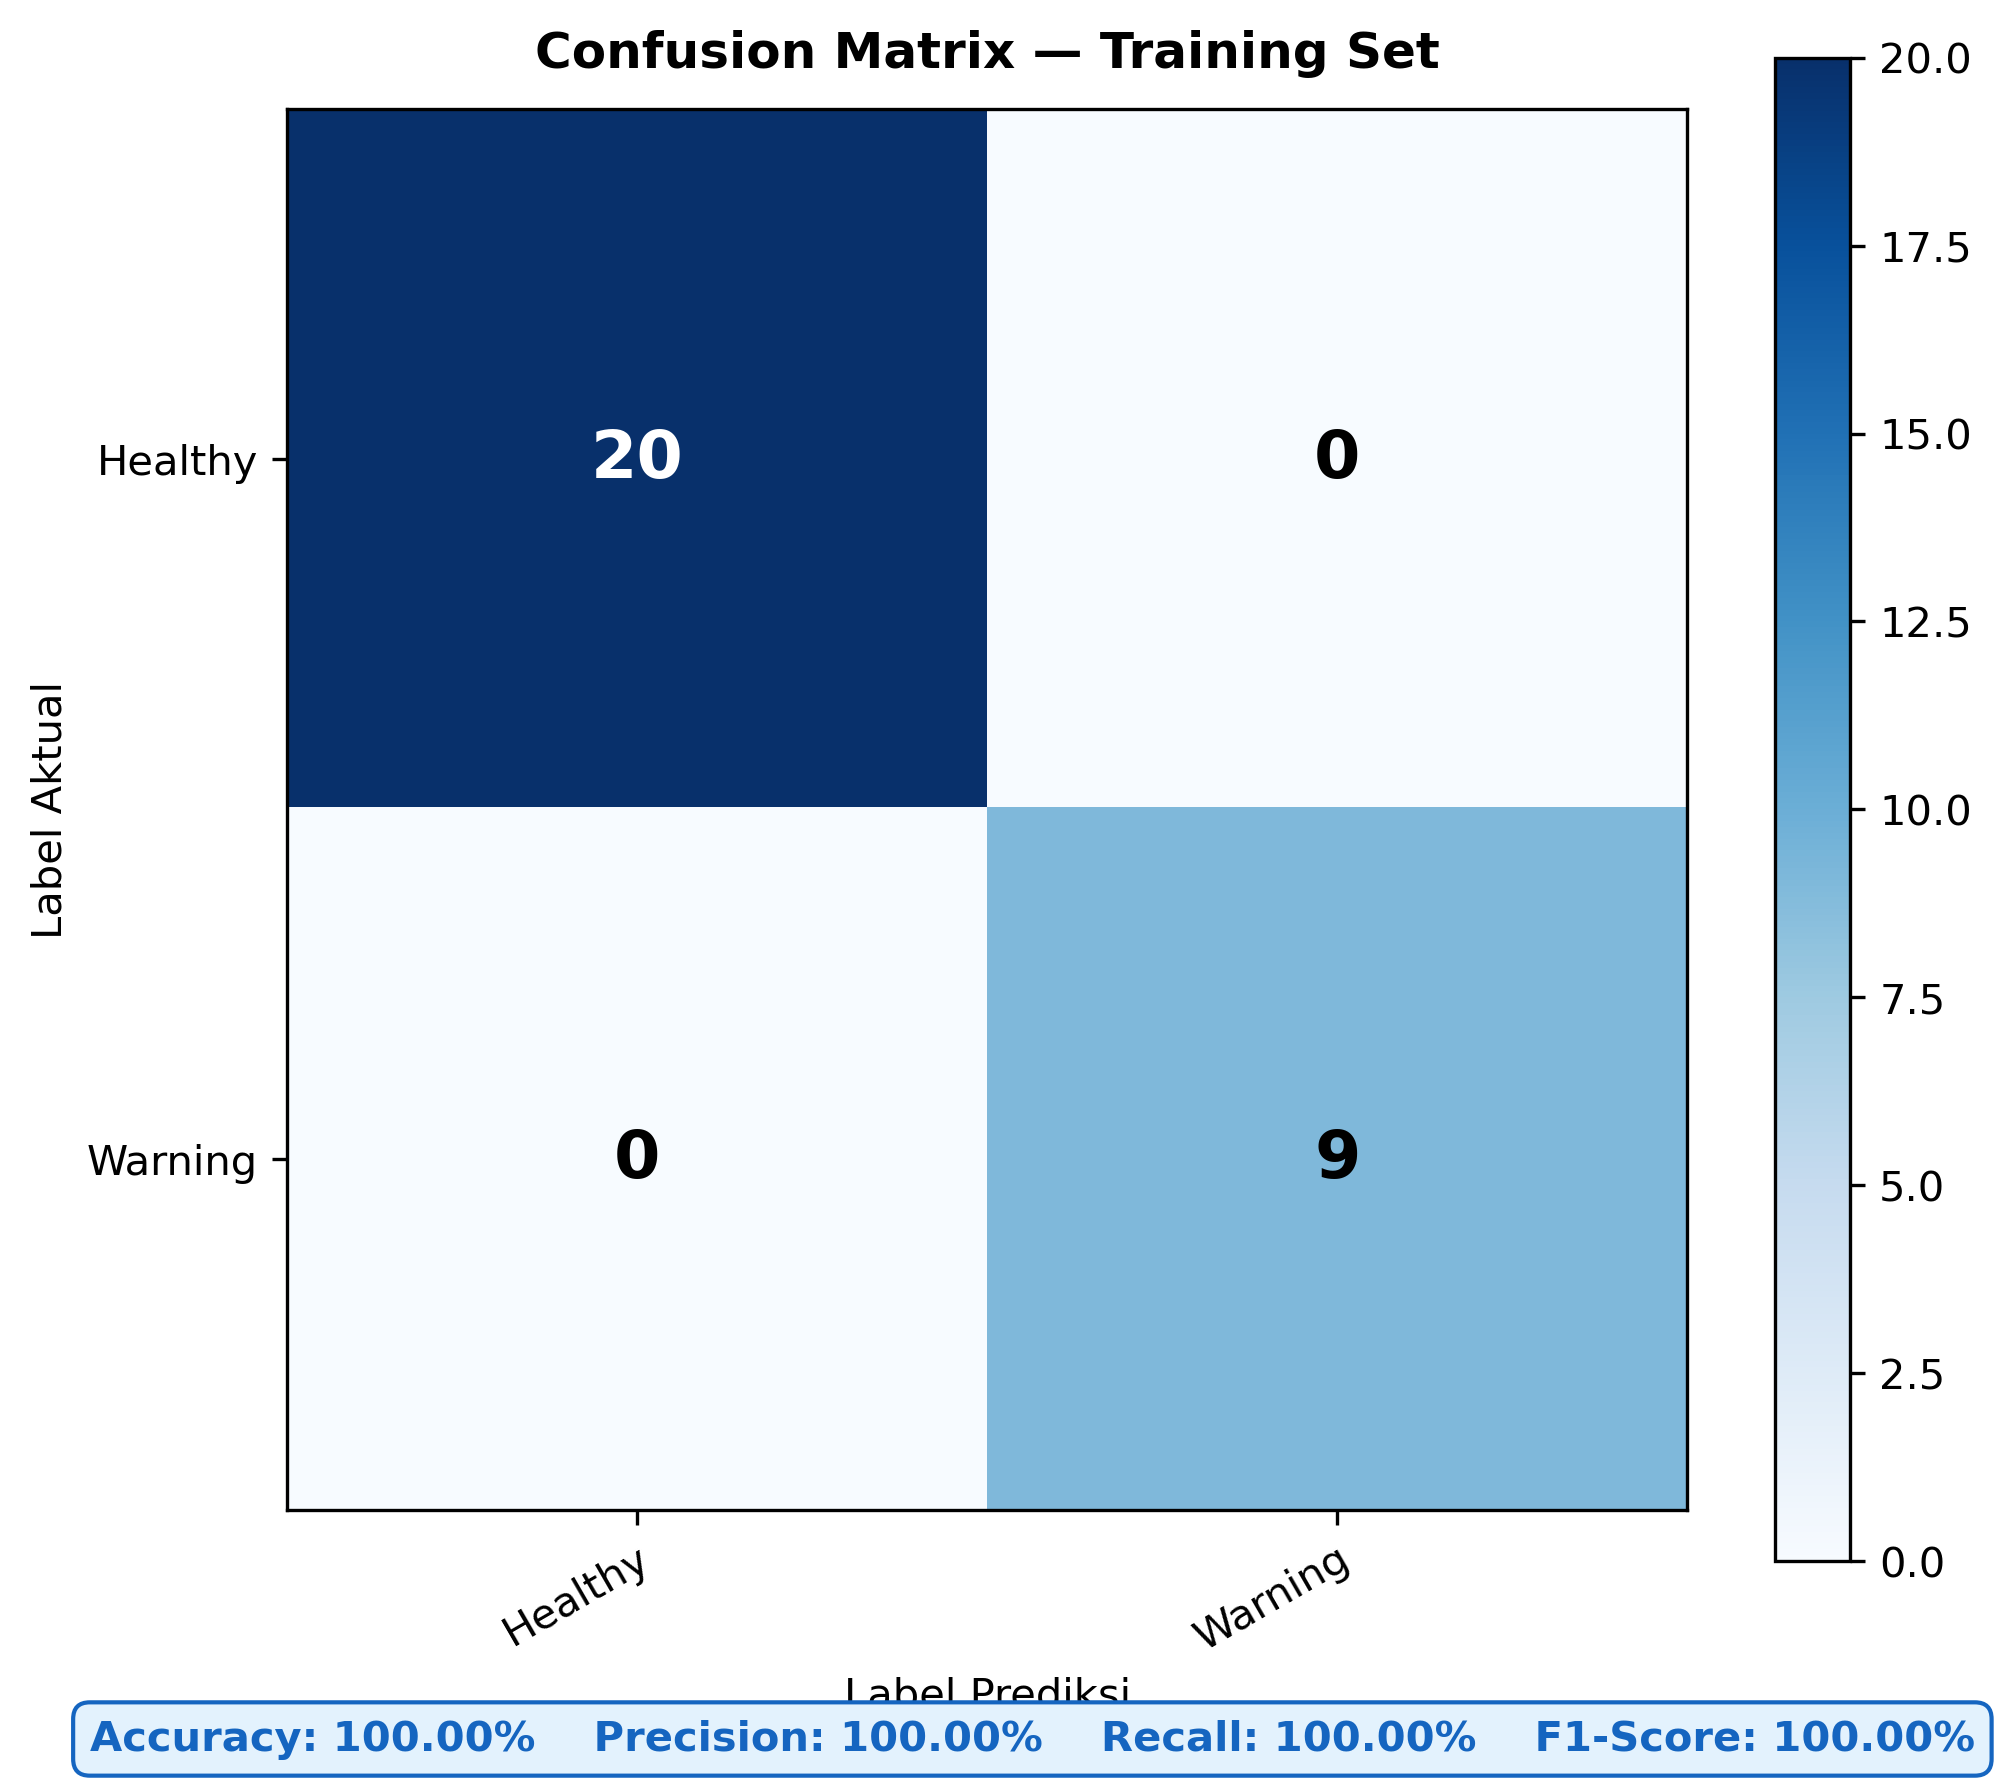
\includegraphics[width=0.85\linewidth]{jurnal_confusion_matrix_train.png}
    \caption{Confusion matrix Training Set — Acc=100.00\%, Prec=100.00\%, Rec=100.00\%, F1=100.00\%.}
    \label{fig:cmtrain}
\end{figure}

\begin{figure}[H]
    \centering
    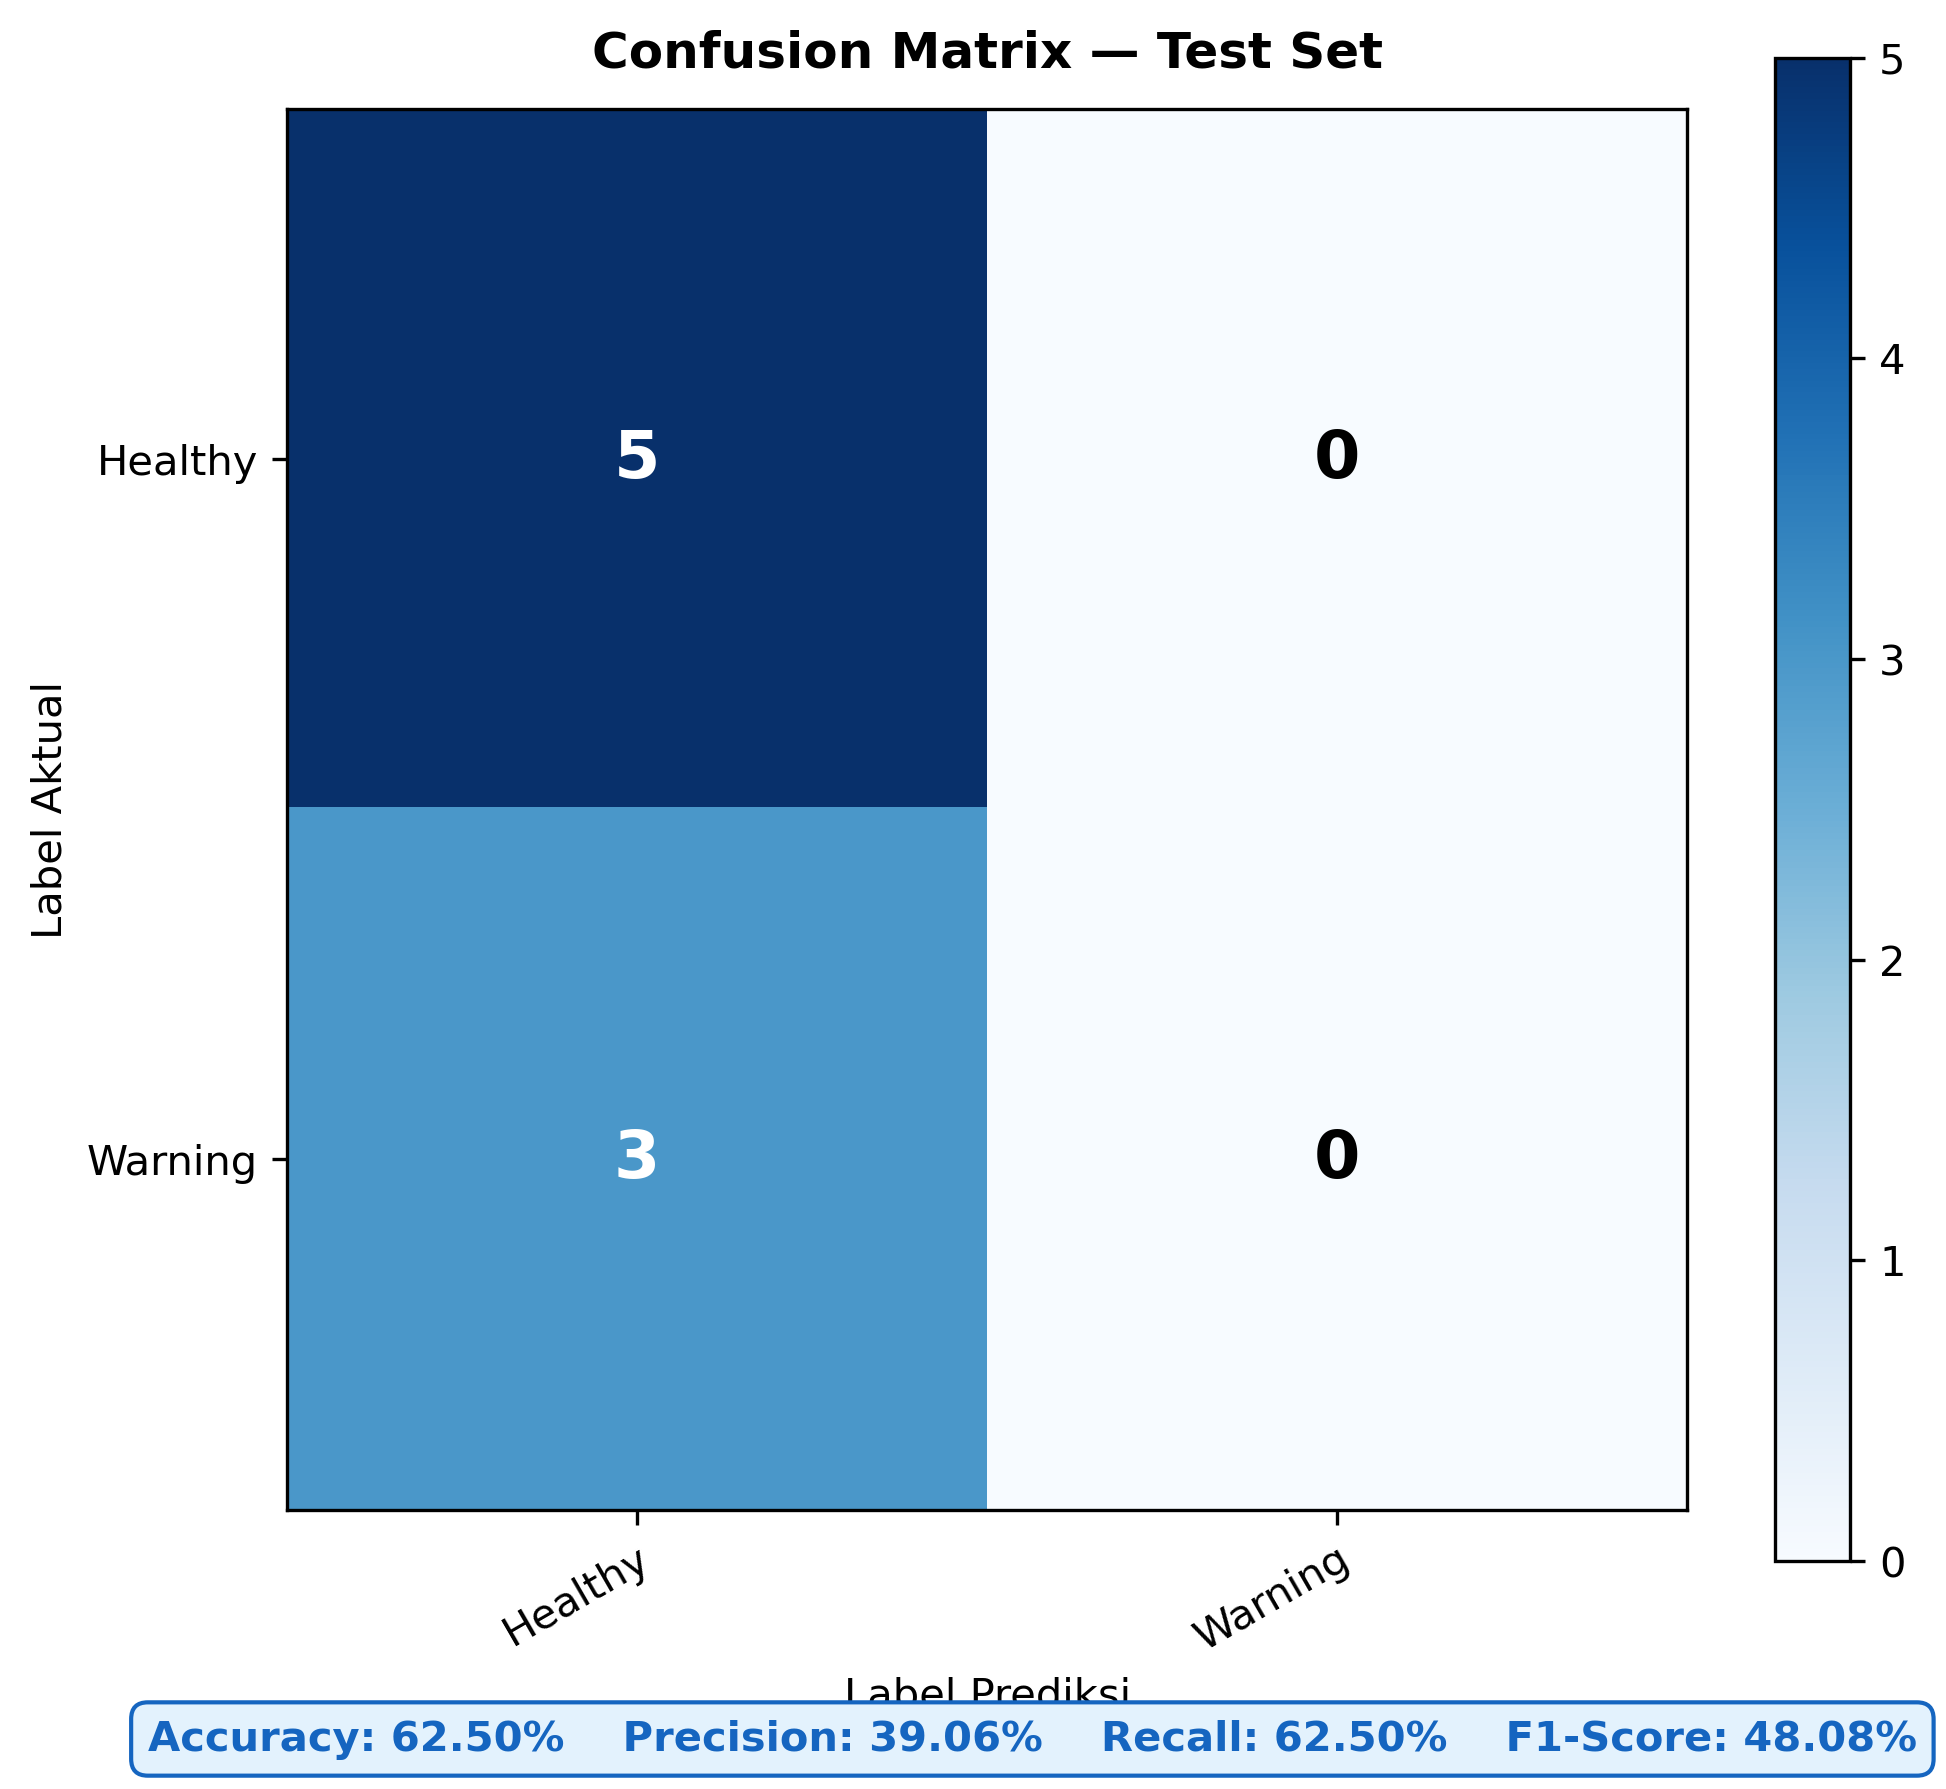
\includegraphics[width=0.85\linewidth]{jurnal_confusion_matrix_test.png}
    \caption{Confusion matrix Test Set — Acc=62.50\%, Prec=39.06\%, Rec=62.50\%, F1=48.08\%.}
    \label{fig:cmtest}
\end{figure}

\begin{figure}[H]
    \centering
    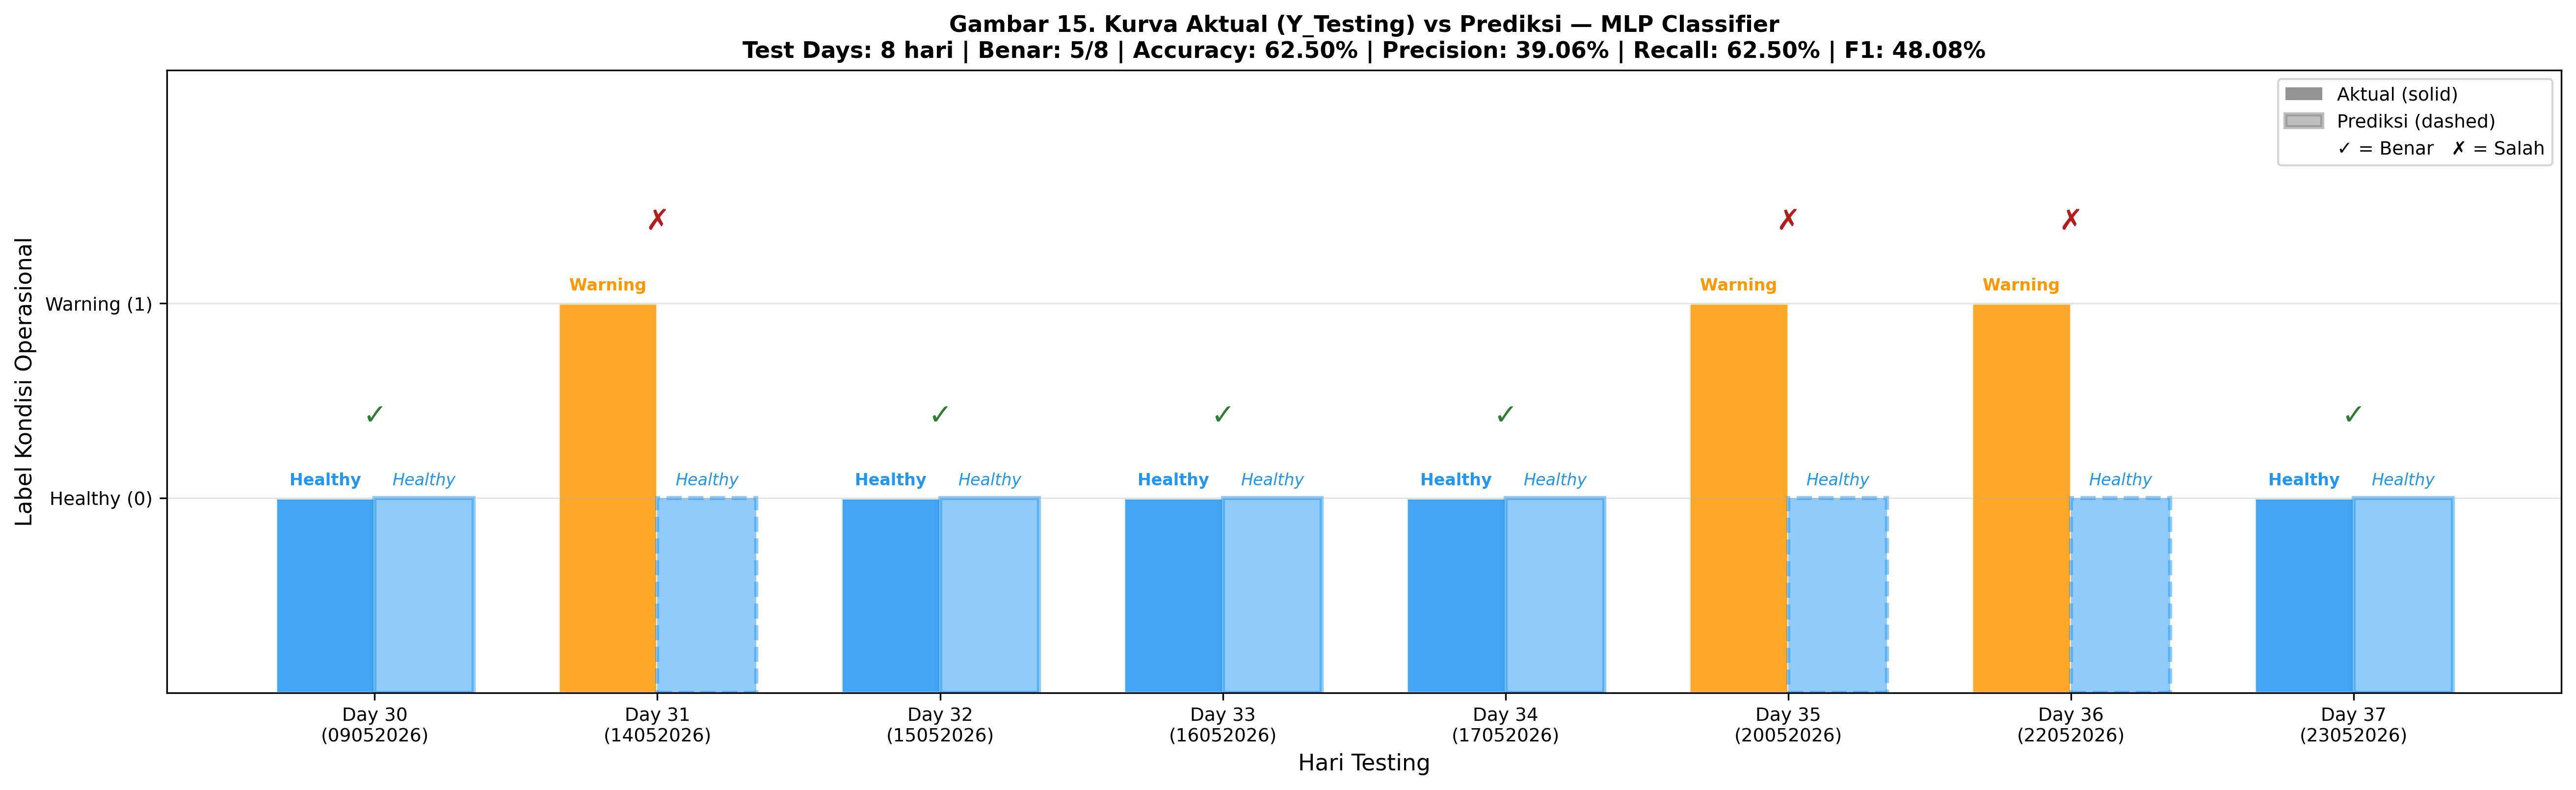
\includegraphics[width=0.85\linewidth]{jurnal_aktual_vs_prediksi_mlp.png}
    \caption{Perbandingan status aktual vs prediksi MLP Classifier per hari.}
    \label{fig:aktualpred}
\end{figure}

\subsection*{Catatan Analisis: Indikasi Overfitting}
Terdapat kesenjangan besar antara performa training (Acc 100\%, CE 0.0002) dan testing (Acc 62.5\%, CE 5.90). Model MLP memprediksi \healthy\ untuk seluruh 8 hari test, sehingga ketiga hari \warning\ aktual (Day 31, 35, 36) seluruhnya salah diklasifikasikan. Penyebab utama yang diduga:
\begin{itemize}
    \item Ukuran dataset klasifikasi sangat kecil (29 sampel training, hanya 9 sampel kelas Warning).
    \item Tidak ada mekanisme \textit{early stopping}; training berjalan penuh 100 epoch dengan learning rate konstan 1e-3.
    \item Model bias ke kelas mayoritas (Healthy) saat menghadapi data test yang belum pernah dilihat.
\end{itemize}

\newpage
% ============================================================
\section{Inference}
% ============================================================

\subsection{Training Inference (dengan Ground Truth)}
\textit{Konsep}: 3 hari terakhir data \textit{training} digunakan untuk memprediksi hari pertama data \textit{testing}, sehingga \textit{ground truth} tersedia dan metrik regresi dapat dihitung.

\begin{table}[H]
    \centering
    \caption{Detail Training Inference.}
    \begin{tabular}{ll}
        \toprule
        \textbf{Keterangan} & \textbf{Nilai} \\
        \midrule
        Input Hari A (Day 27) & 06052026 — \warning \\
        Input Hari B (Day 28) & 07052026 — \healthy \\
        Input Hari C (Day 29) & 08052026 — \healthy \\
        Target Hari D (Day 30) & 09052026 \\
        Prediksi Status & \healthy\ (99.96\% confidence) \\
        Prob. Healthy & 99.96\% \\
        Prob. Warning & 0.04\% \\
        Status Aktual & \healthy \\
        Klasifikasi & \ok\ BENAR \\
        MSE Prediksi vs Aktual & 0.00495024 (0.4950\%) \\
        RMSE & 0.07035795 \\
        MAE & 0.03708208 \\
        \bottomrule
    \end{tabular}
\end{table}

\begin{figure}[H]
    \centering
    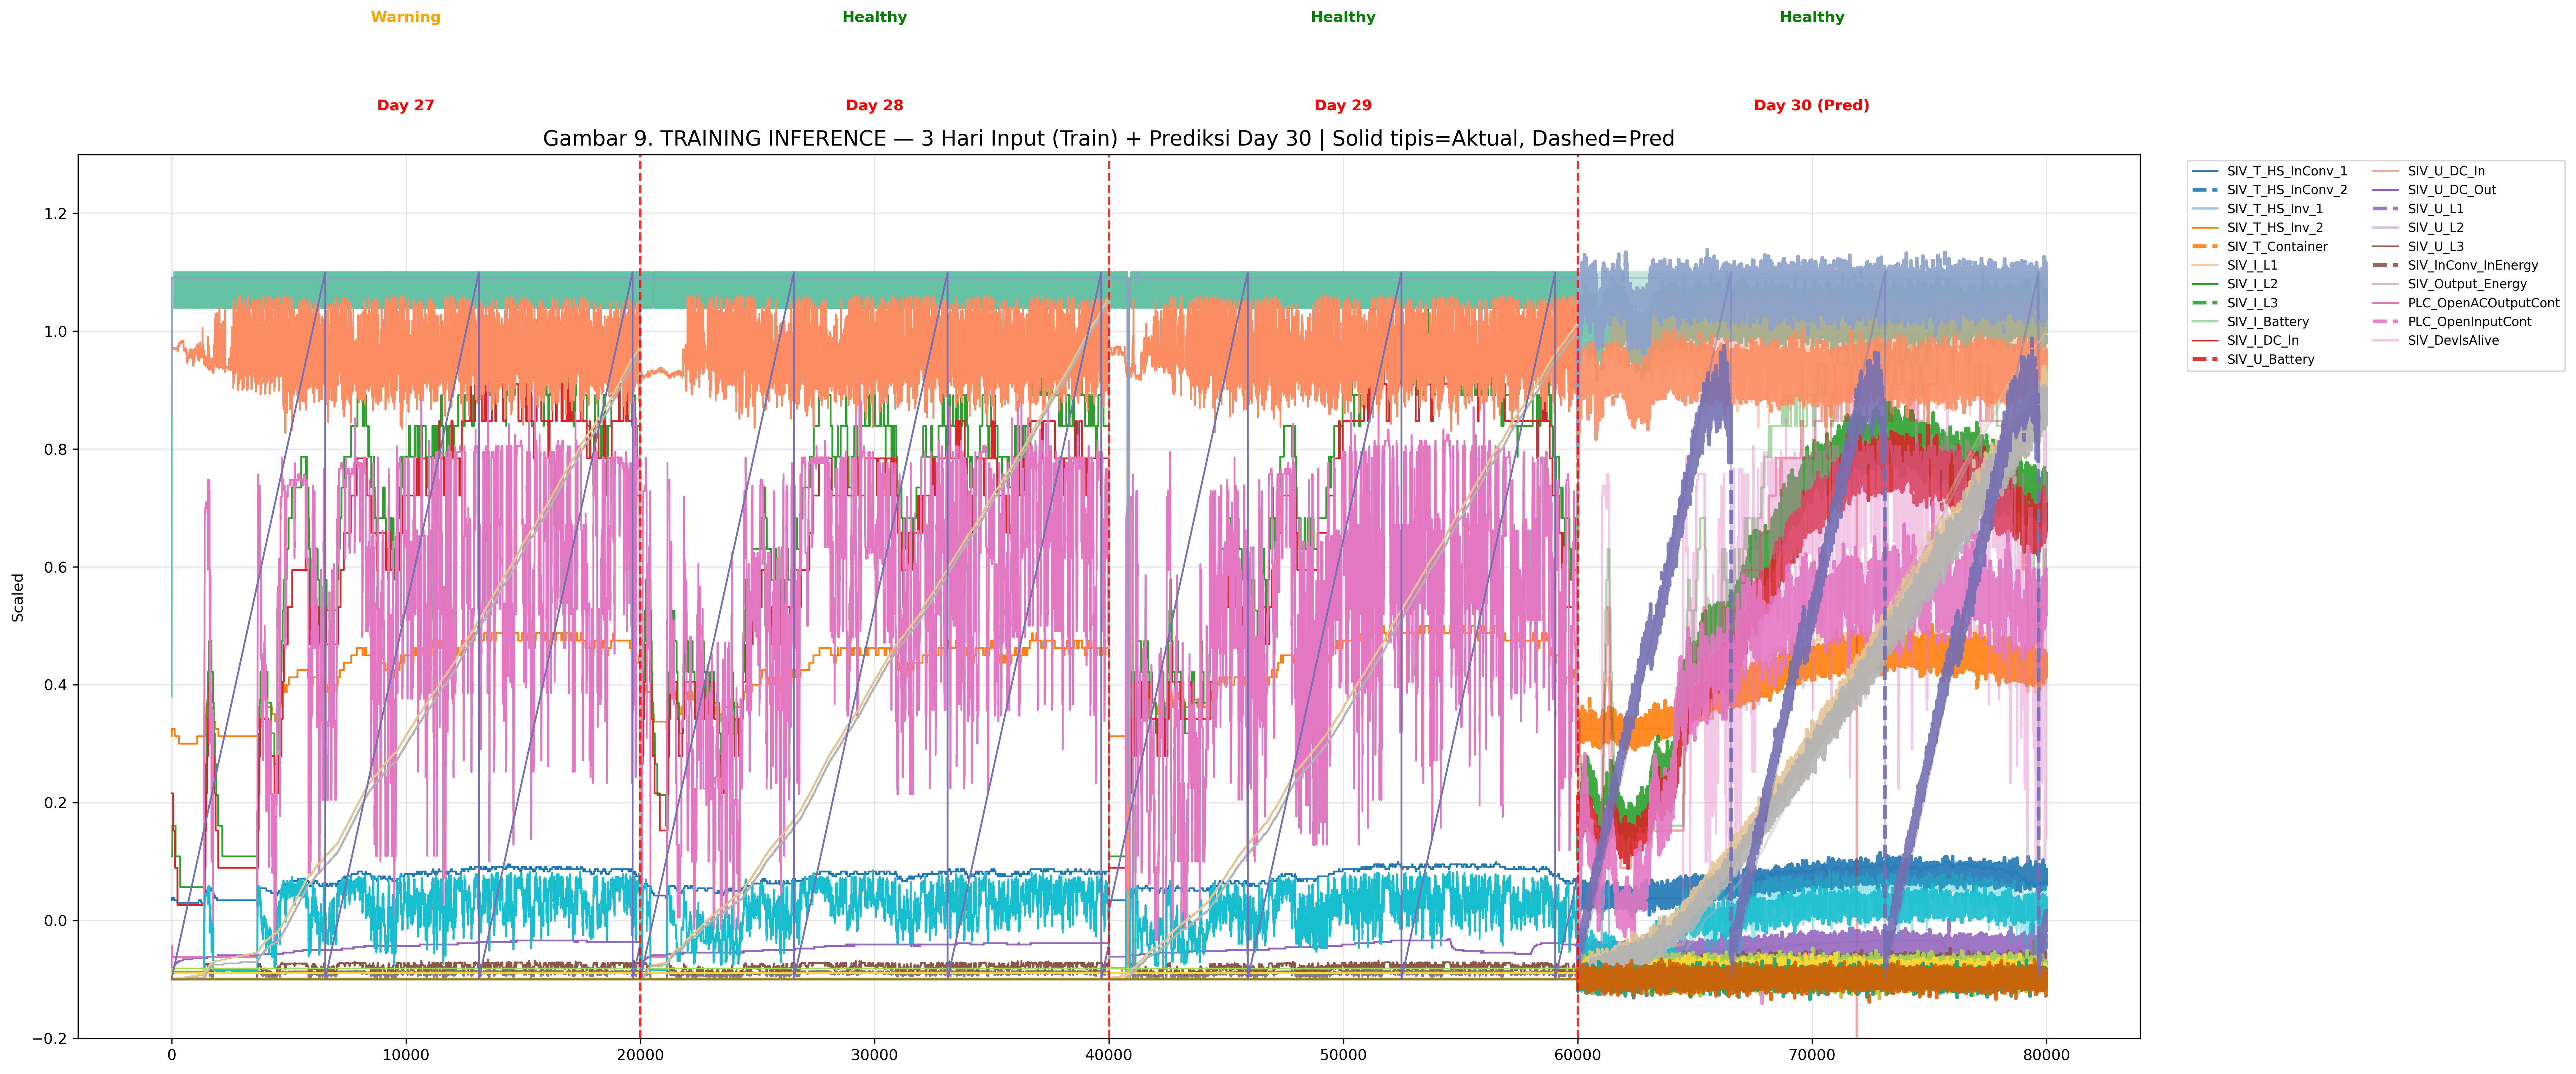
\includegraphics[width=0.85\linewidth]{gambar_train1_input_prediksi.png}
    \caption{Training Inference — 3 hari input training + hasil prediksi (supplementary).}
    \label{fig:traininput}
\end{figure}

\begin{figure}[H]
    \centering
    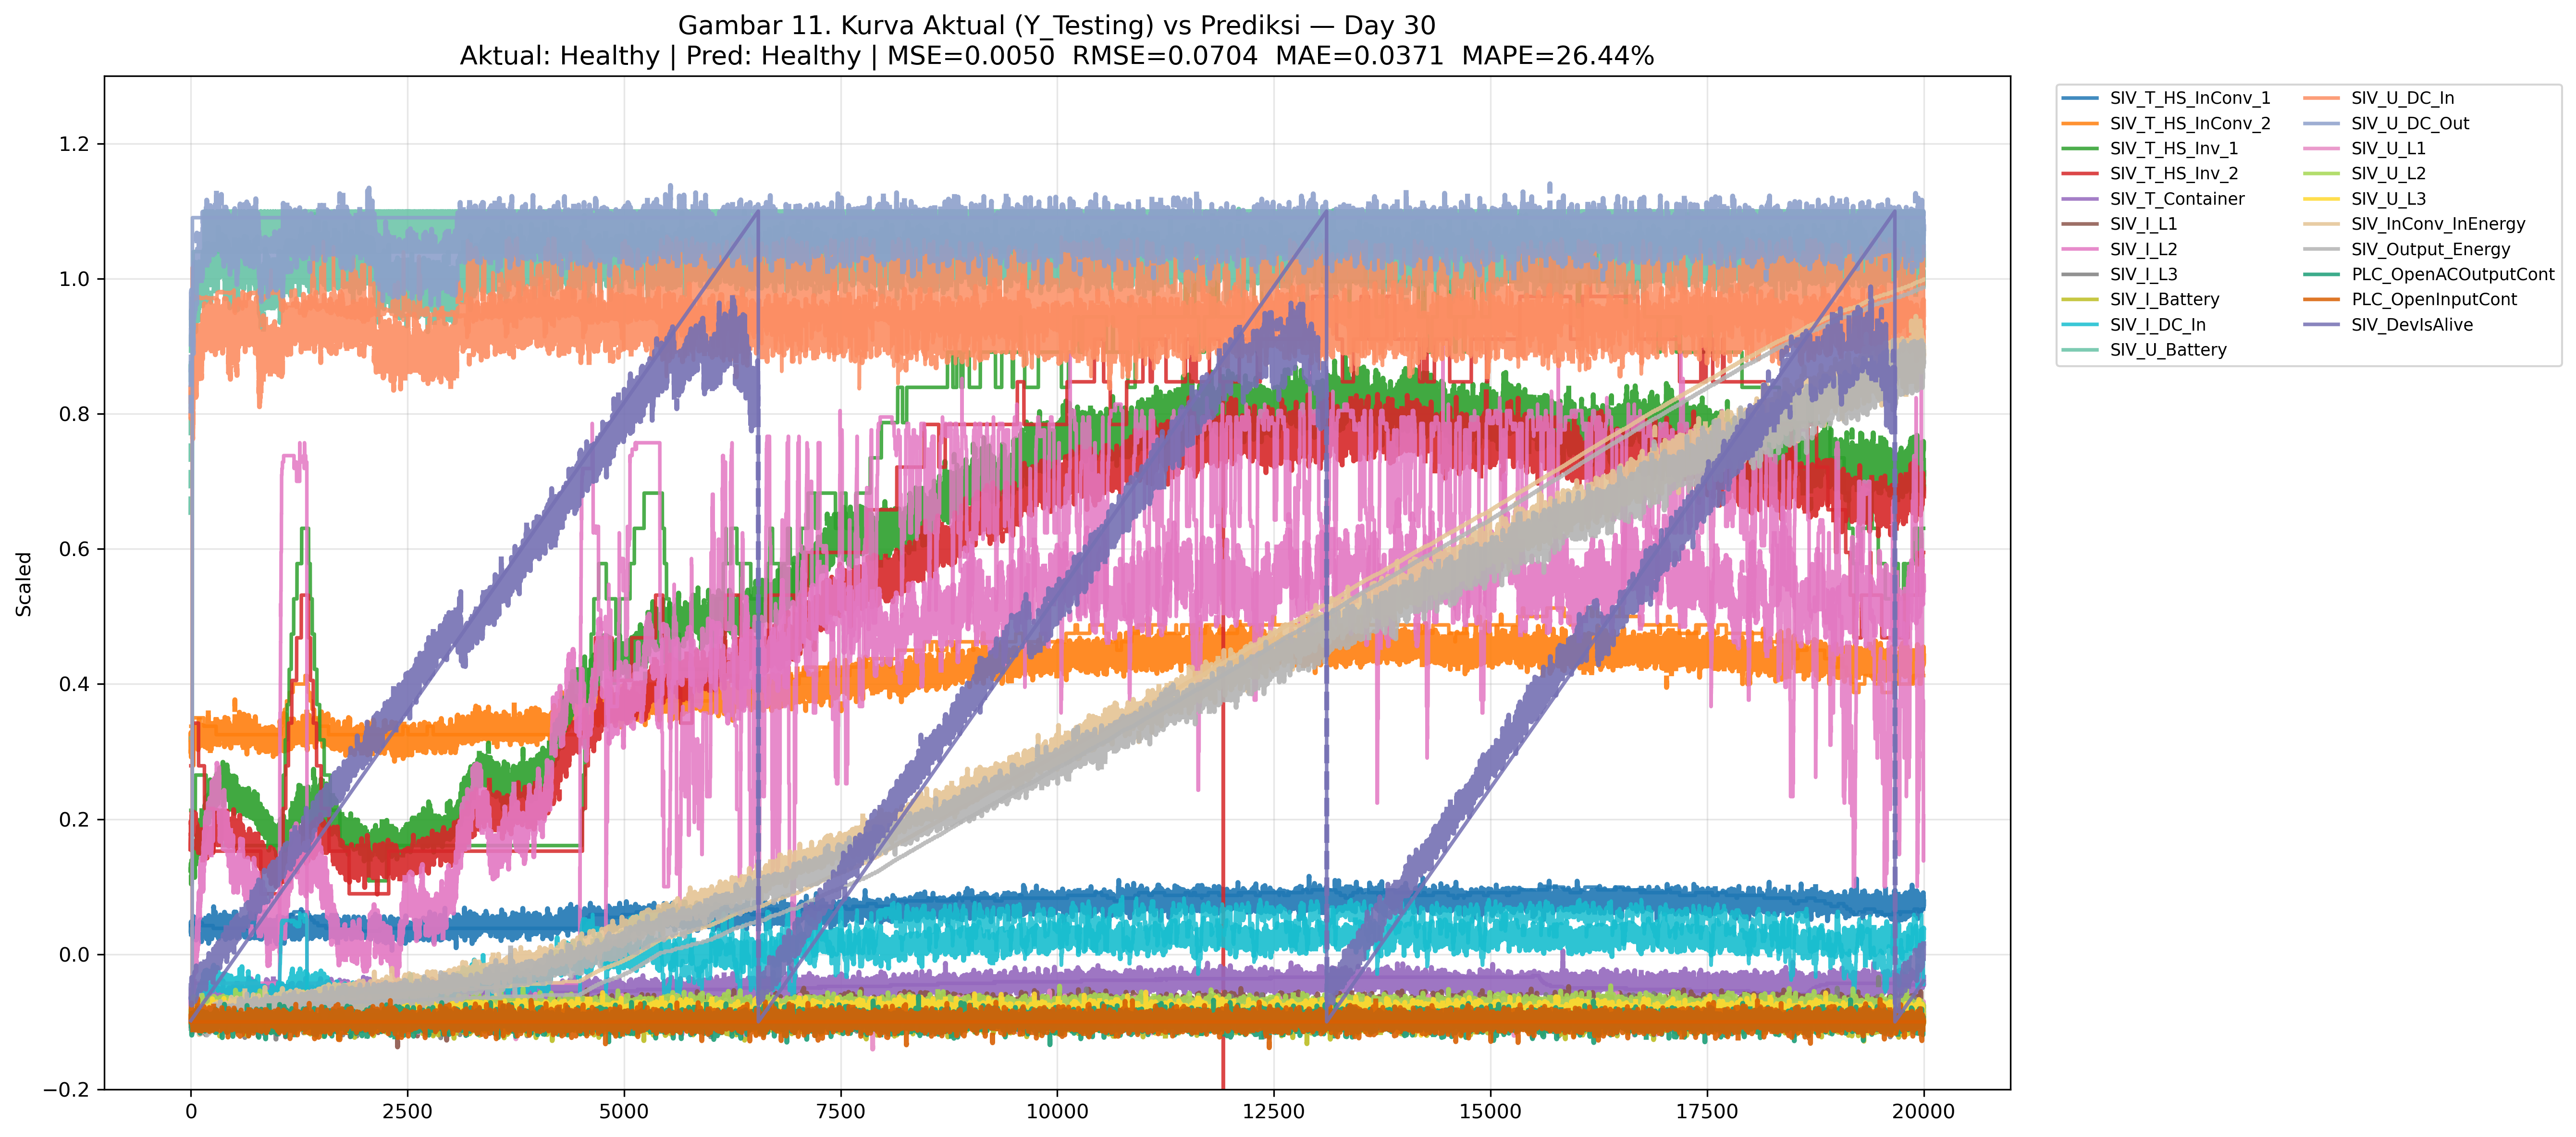
\includegraphics[width=0.85\linewidth]{gambar_train2_real_vs_pred.png}
    \caption{Training Inference — perbandingan aktual (Y\_Testing) vs prediksi.}
    \label{fig:trainrealpred}
\end{figure}

\subsection{Testing Inference (tanpa Ground Truth)}
\textit{Konsep}: 3 hari terakhir data \textit{testing} (hari-hari terakhir dataset) digunakan untuk memprediksi hari ke-38 (masa depan), sehingga tidak ada \textit{ground truth} dan metrik regresi tidak dapat dihitung.

\begin{table}[H]
    \centering
    \caption{Detail Testing Inference (forecasting masa depan).}
    \begin{tabular}{ll}
        \toprule
        \textbf{Keterangan} & \textbf{Nilai} \\
        \midrule
        Input Hari A (Day 35) & 20052026 — \warning \\
        Input Hari B (Day 36) & 22052026 — \warning \\
        Input Hari C (Day 37) & 23052026 — \healthy \\
        Target & Hari ke-38 (masa depan) \\
        Prediksi Status & \healthy \\
        Confidence & 99.96\% \\
        Prob. Healthy & 99.96\% \\
        Prob. Warning & 0.04\% \\
        Ground Truth & Tidak tersedia \\
        Metrik MSE/RMSE/MAE & Tidak dapat dihitung \\
        \bottomrule
    \end{tabular}
\end{table}

\begin{figure}[H]
    \centering
    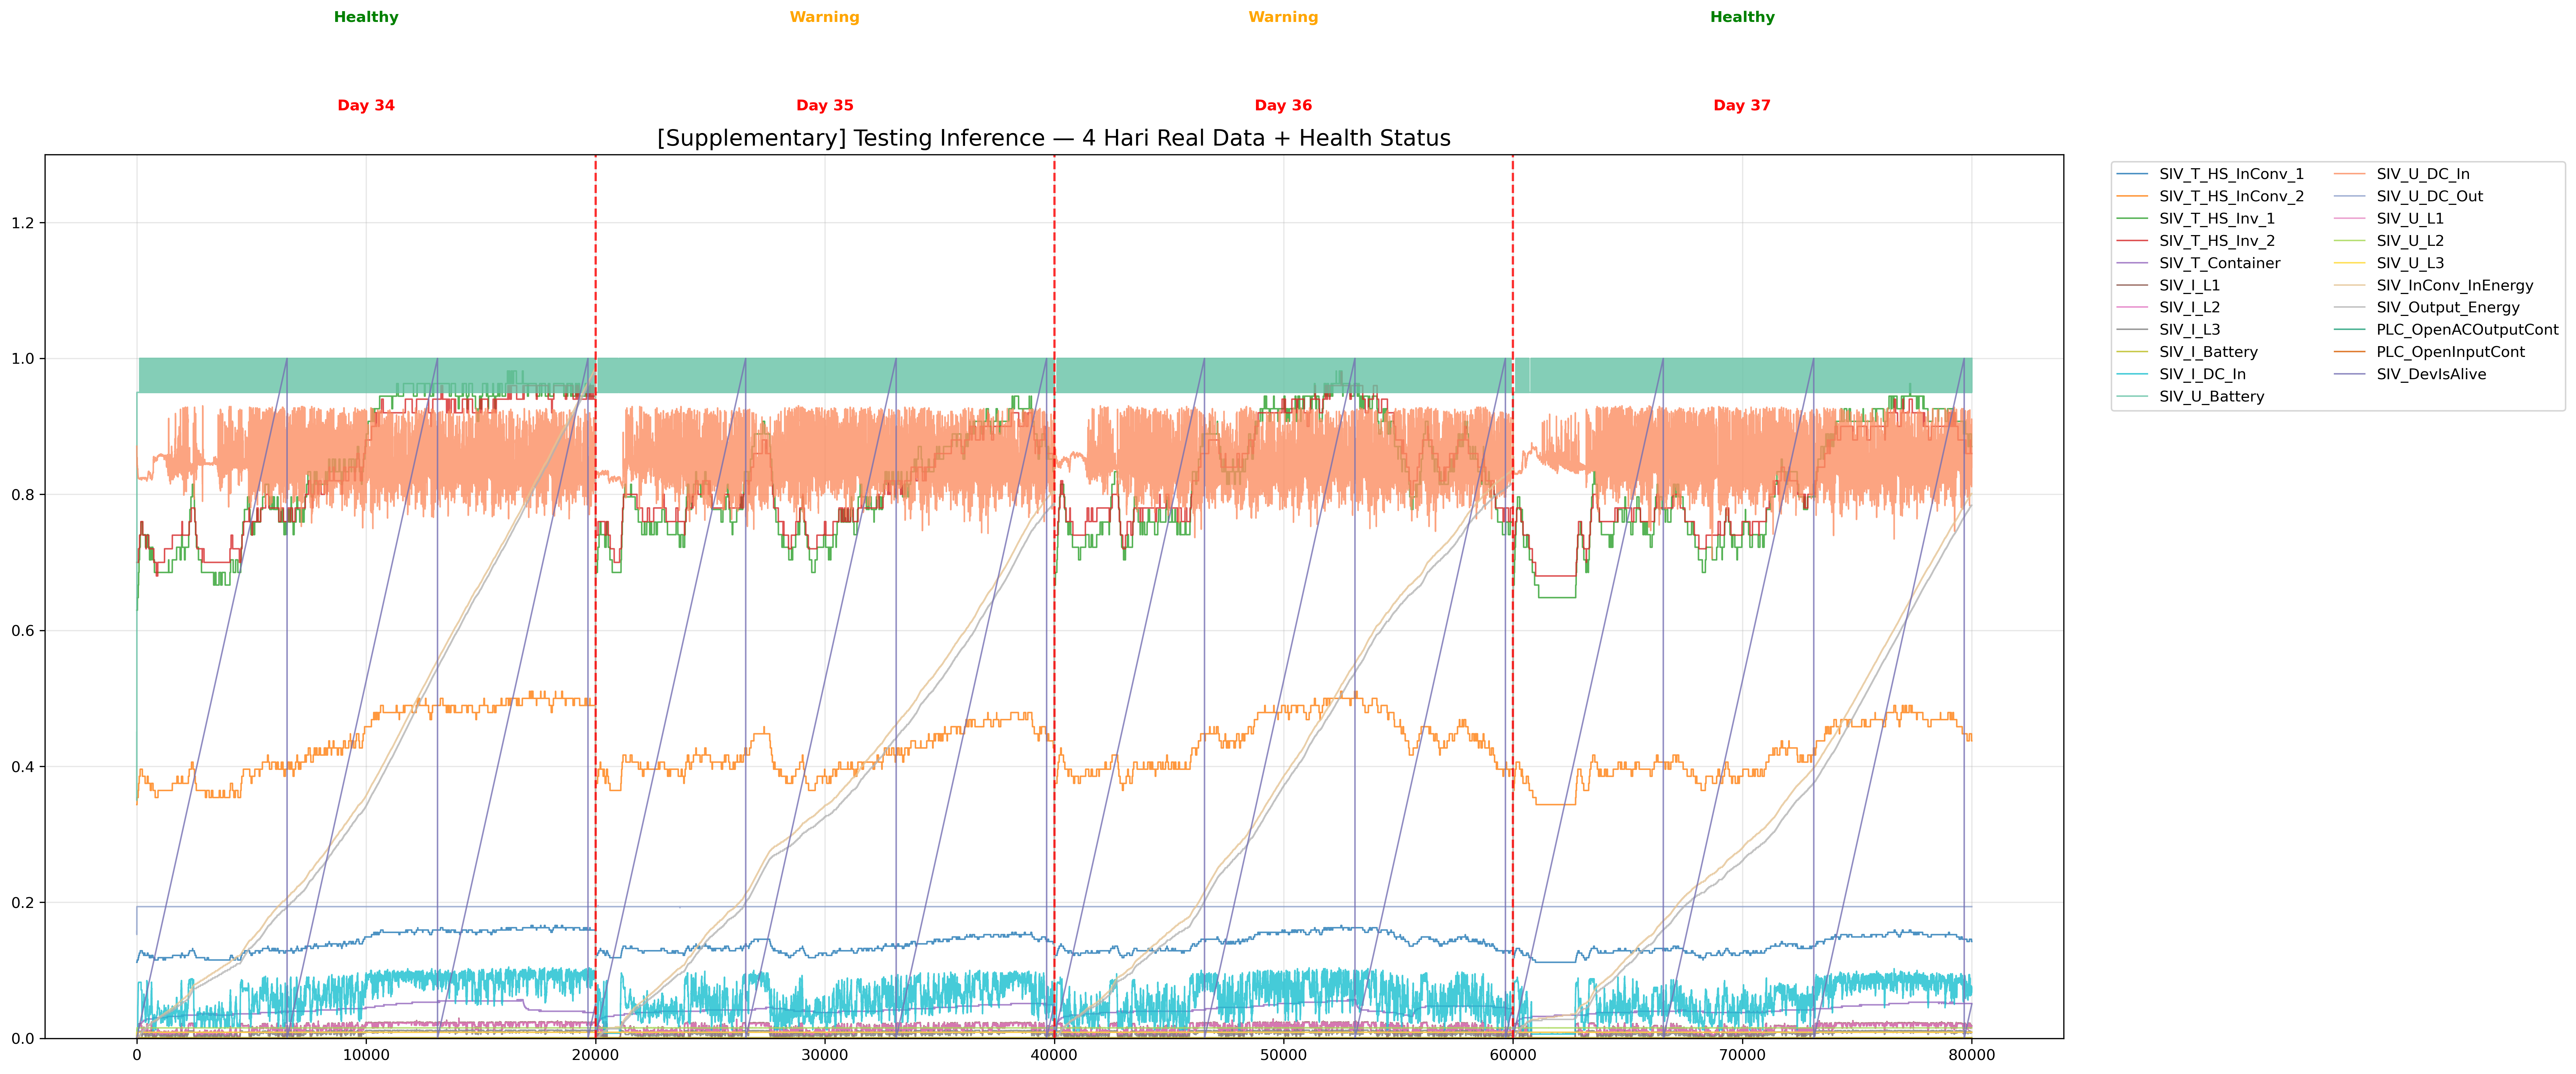
\includegraphics[width=0.85\linewidth]{gambar1_4hari_real_TCN.png}
    \caption{Konteks 4 hari data real menjelang Testing Inference (supplementary).}
    \label{fig:4hari}
\end{figure}

\begin{figure}[H]
    \centering
    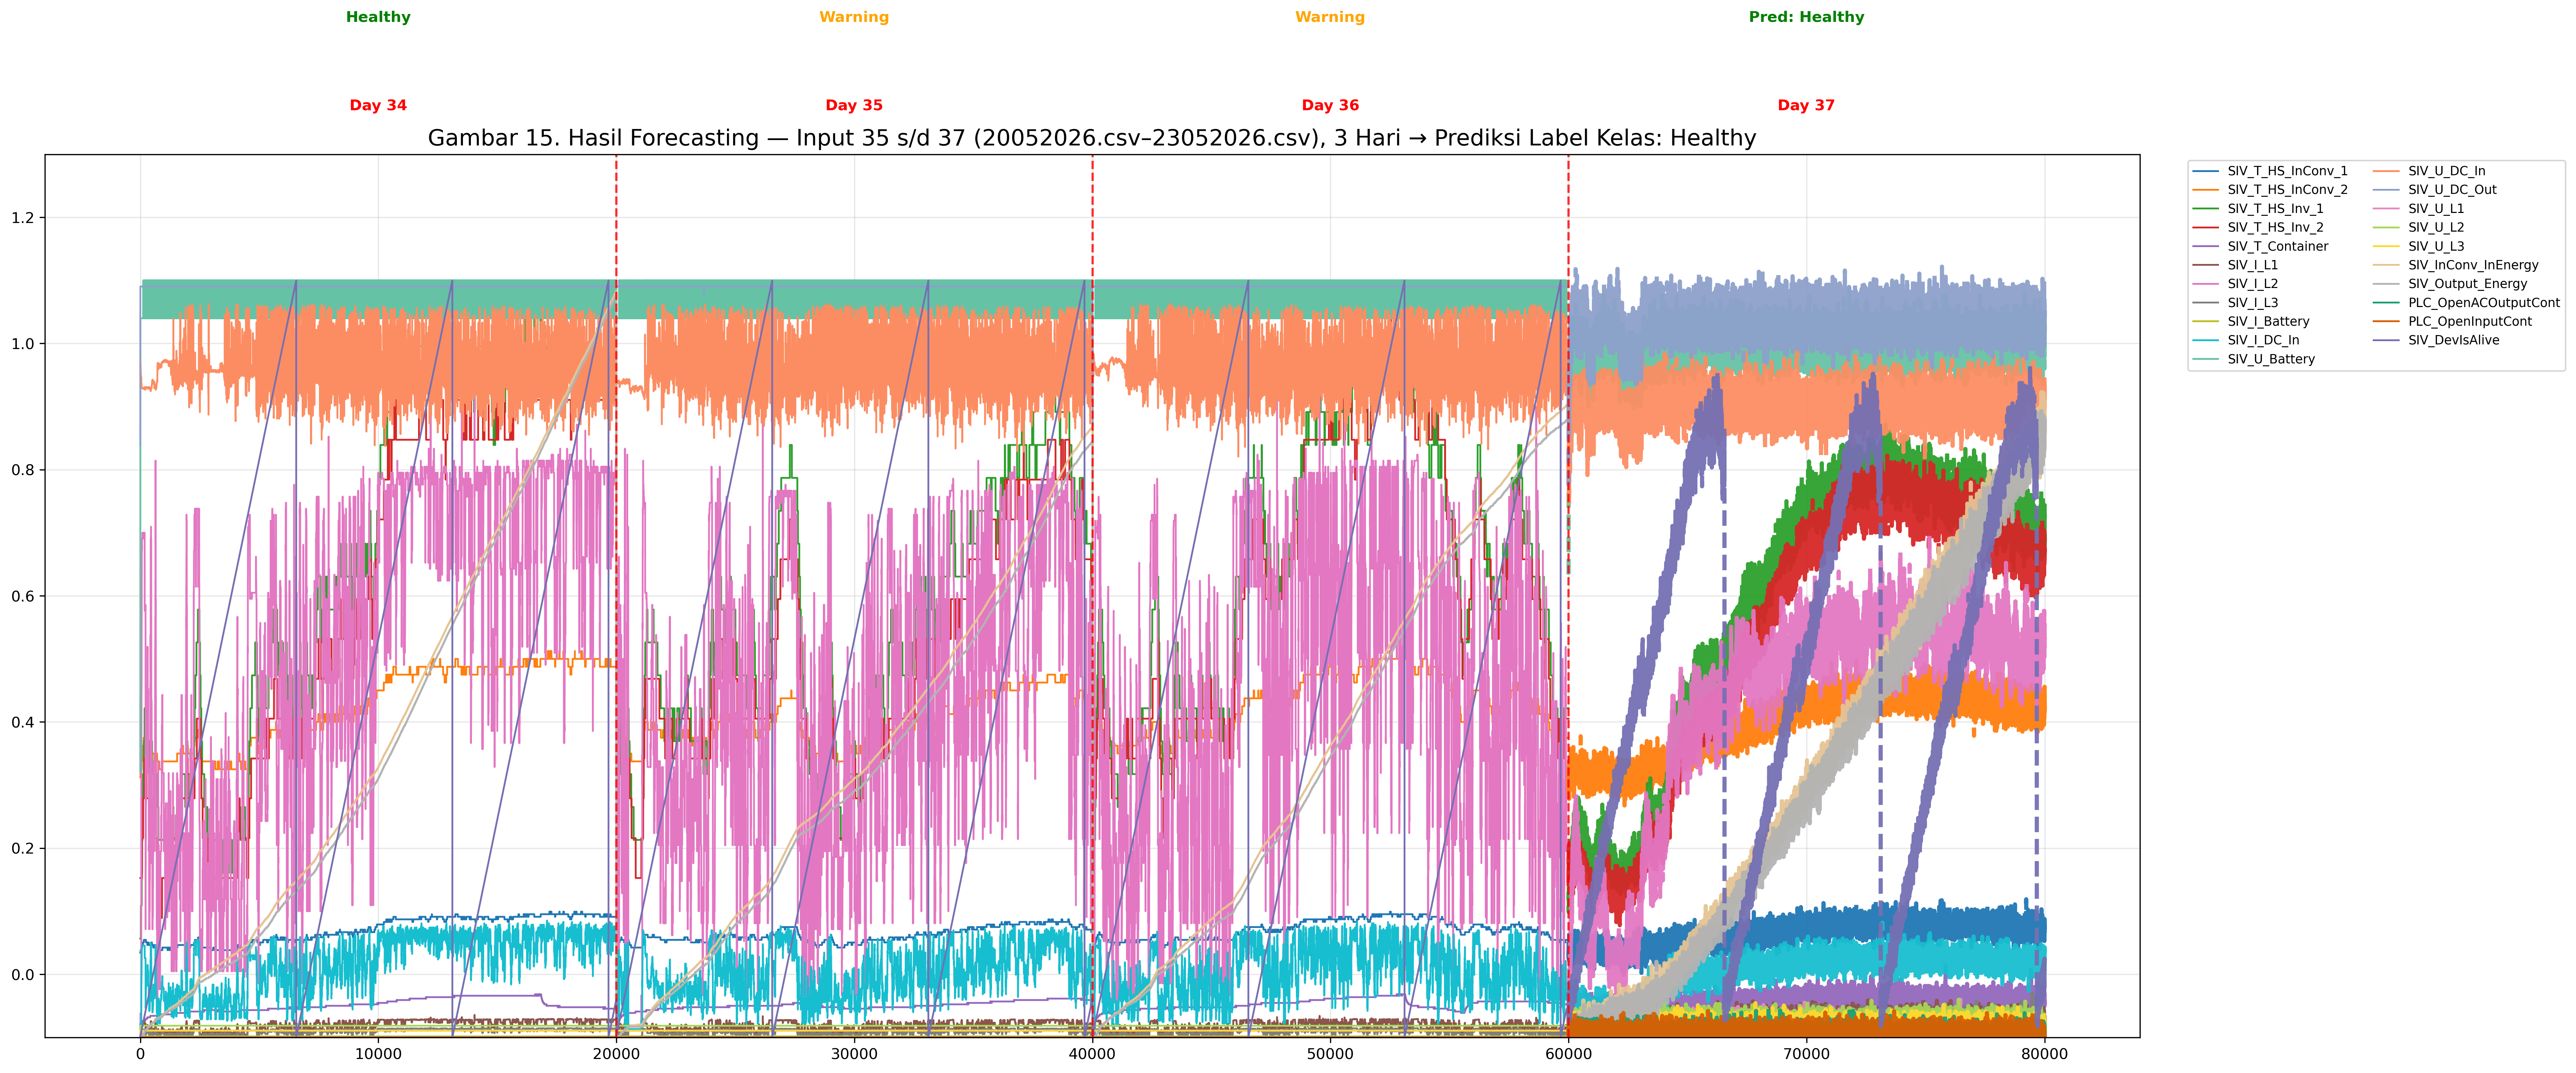
\includegraphics[width=0.85\linewidth]{gambar2_input_plus_prediksi_TCN.png}
    \caption{Testing Inference — hasil forecasting hari ke-38 beserta label kelas prediksi.}
    \label{fig:testforecast}
\end{figure}

\begin{figure}[H]
    \centering
    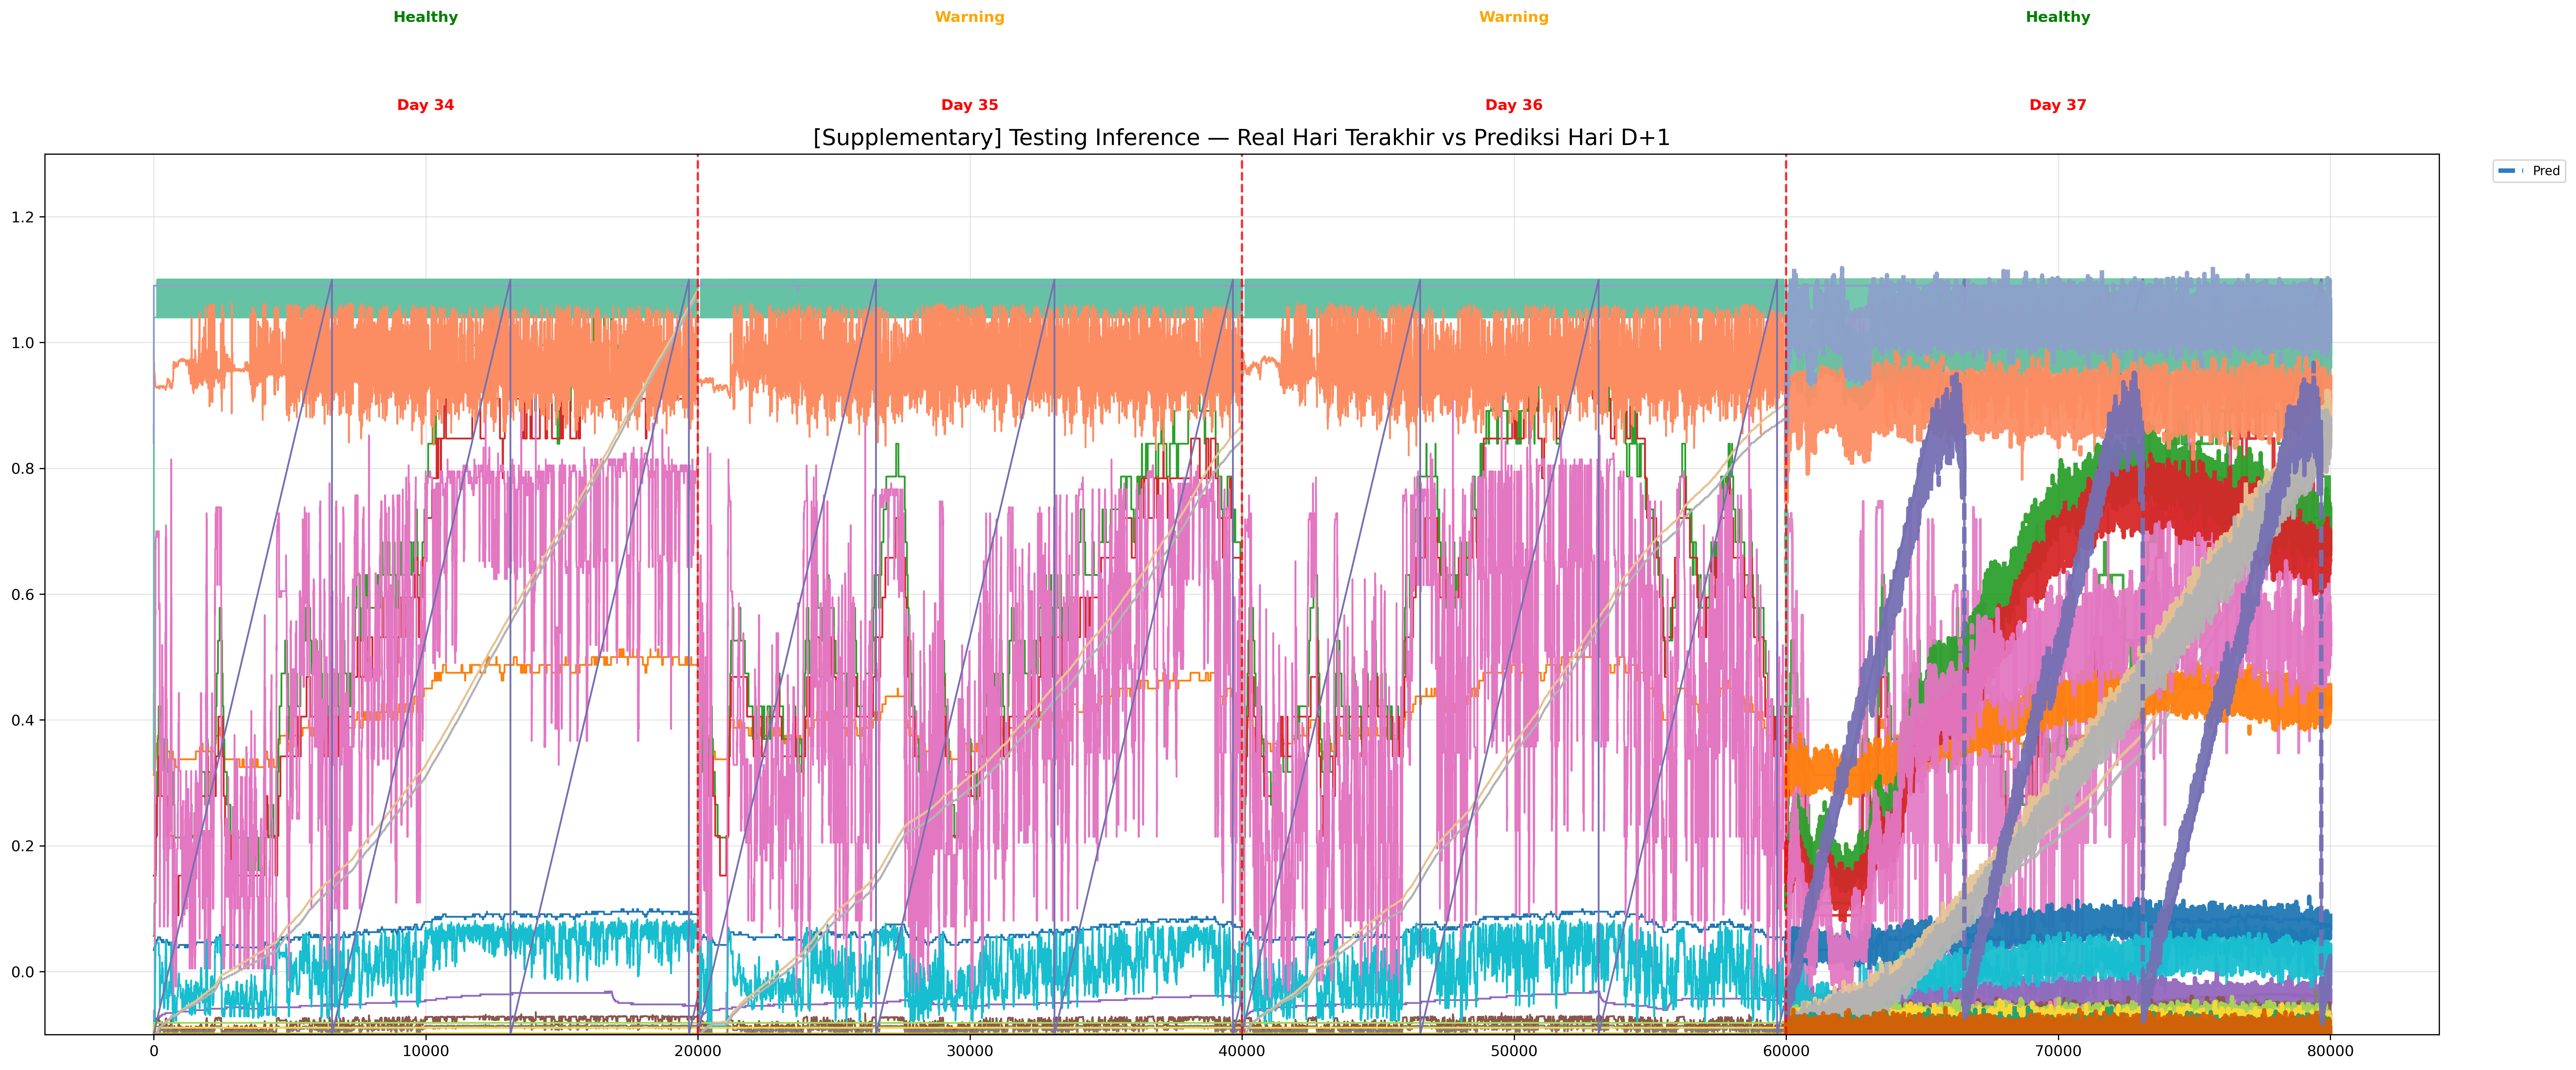
\includegraphics[width=0.85\linewidth]{gambar3_real_vs_prediksi_TCN.png}
    \caption{Overlay data real vs prediksi pada Testing Inference (supplementary).}
    \label{fig:testrealpred}
\end{figure}

\subsection{Perbandingan Training Inference vs Testing Inference}
\begin{table}[H]
    \centering
    \small
    \caption{Perbandingan Training Inference vs Testing Inference.}
    \begin{tabular}{lll}
        \toprule
        \textbf{Aspek} & \textbf{Training Inference} & \textbf{Testing Inference} \\
        \midrule
        Input Days & Day 27--29 (Train) & Day 35--37 (Test) \\
        Target & Day 30 (1st Test) & Day 38 (Future) \\
        Prediksi Status & \healthy\ (100.0\%) & \healthy\ (100.0\%) \\
        Ground Truth & \healthy & Tidak ada \\
        Klasifikasi Benar? & \ok\ BENAR & Tidak dapat diukur \\
        MSE & 0.004950 & Tidak dapat diukur \\
        RMSE & 0.070358 & Tidak dapat diukur \\
        MAE & 0.037082 & Tidak dapat diukur \\
        \bottomrule
    \end{tabular}
\end{table}

\noindent\textbf{Kesimpulan Inference:}
\begin{itemize}
    \item Training Inference memiliki metrik kuantitatif (MSE/RMSE/MAE) karena hari yang diprediksi (D+1) sudah memiliki data sebagai \textit{ground truth}.
    \item Testing Inference hanya memiliki \textit{confidence score} karena memprediksi hari masa depan yang belum memiliki data. Akurasi tidak dapat diukur secara kuantitatif.
    \item Kedua inference menggunakan model yang sama (hasil training Stage 1 \& Stage 2). Perbedaan hanya pada data input dan ketersediaan \textit{ground truth}.
\end{itemize}

\newpage
% ============================================================
\section{Ringkasan dan Kesimpulan}
% ============================================================

\begin{table}[H]
    \centering
    \caption{Ringkasan performa akhir kedua tahap model.}
    \begin{tabular}{lll}
        \toprule
        \textbf{Model} & \textbf{Metrik Utama} & \textbf{Train / Test} \\
        \midrule
        Stage 1 — TCN Forecaster & MSE & 0.008066 / 0.007446 \\
                                  & RMSE & 0.089810 / 0.086292 \\
                                  & MAE & 0.046303 / 0.043340 \\
        Stage 2 — MLP Classifier & Accuracy & 100.00\% / 62.50\% \\
                                  & F1-Score & 100.00\% / 48.08\% \\
        \bottomrule
    \end{tabular}
\end{table}

\begin{enumerate}
    \item \textbf{Stage 1 (TCN Forecaster)} menunjukkan performa yang \textbf{baik dan stabil}, dengan selisih MSE train--test yang kecil (0.00456), mengindikasikan kemampuan generalisasi yang memadai terhadap sinyal sensor yang belum pernah dilihat model.
    \item \textbf{Stage 2 (MLP Classifier)} menunjukkan \textbf{indikasi overfitting yang signifikan} — akurasi training sempurna (100\%) namun akurasi test jatuh ke 62.5\%, dengan model gagal mendeteksi seluruh kasus \warning\ pada data test (recall Warning = 0\%).
    \item Penyebab utama overfitting Stage 2 kemungkinan besar adalah \textbf{ukuran dataset klasifikasi yang sangat kecil} (29 hari training, hanya 9 sampel kelas Warning) relatif terhadap kompleksitas model (84 input $\to$ 256 $\to$ 128 $\to$ 64 $\to$ 2) dan jumlah epoch (100) tanpa \textit{early stopping}.
    \item \textbf{Rekomendasi perbaikan}: (a) menambah jumlah data harian berlabel, (b) menerapkan \textit{early stopping} berbasis validation loss, (c) mengurangi kapasitas model atau menambah regularisasi (dropout/weight decay lebih besar), (d) mempertimbangkan teknik augmentasi data atau \textit{k-fold cross-validation} mengingat ukuran dataset yang terbatas.
\end{enumerate}

\newpage
% ============================================================
\section{Lampiran — Daftar File Output}
% ============================================================

\begin{table}[H]
    \centering
    \small
    \caption{Daftar seluruh file gambar hasil eksperimen (folder \texttt{evidence/}).}
    \begin{tabular}{ll}
        \toprule
        \textbf{Nama File} & \textbf{Deskripsi} \\
        \midrule
        jurnal\_flowchart\_stage1.png & Pipeline TCN (Gambar~\ref{fig:flow1}) \\
        jurnal\_flowchart\_stage2.png & Pipeline MLP (Gambar~\ref{fig:flow2}) \\
        plot\_all\_parameters\_TCN.png & 21 parameter seluruh hari (Gambar~\ref{fig:allparam}) \\
        jurnal\_normalisasi\_comparison.png & Sebelum vs sesudah normalisasi (Gambar~\ref{fig:norm}) \\
        jurnal\_sliding\_window.png & Skema sliding window 3$\to$1 hari (Gambar~\ref{fig:slidewin}) \\
        jurnal\_kurva\_loss\_stage1.png & Kurva Epoch vs MSE Stage 1 (Gambar~\ref{fig:loss1}) \\
        jurnal\_kurva\_loss\_acc\_stage2.png & Kurva CE Loss + Accuracy Stage 2 (Gambar~\ref{fig:loss2}) \\
        jurnal\_confusion\_matrix\_train.png & Confusion matrix training (Gambar~\ref{fig:cmtrain}) \\
        jurnal\_confusion\_matrix\_test.png & Confusion matrix testing (Gambar~\ref{fig:cmtest}) \\
        jurnal\_aktual\_vs\_prediksi\_mlp.png & Aktual vs prediksi MLP (Gambar~\ref{fig:aktualpred}) \\
        gambar\_train1\_input\_prediksi.png & Training Inference — input (Gambar~\ref{fig:traininput}) \\
        gambar\_train2\_real\_vs\_pred.png & Training Inference — real vs pred (Gambar~\ref{fig:trainrealpred}) \\
        gambar1\_4hari\_real\_TCN.png & Konteks 4 hari real testing (Gambar~\ref{fig:4hari}) \\
        gambar2\_input\_plus\_prediksi\_TCN.png & Testing Inference — forecasting (Gambar~\ref{fig:testforecast}) \\
        gambar3\_real\_vs\_prediksi\_TCN.png & Testing Inference — overlay (Gambar~\ref{fig:testrealpred}) \\
        \bottomrule
    \end{tabular}
\end{table}

\begin{table}[H]
    \centering
    \caption{Daftar file data numerik dan model.}
    \begin{tabular}{ll}
        \toprule
        \textbf{Nama File} & \textbf{Deskripsi} \\
        \midrule
        jurnal\_info\_stage1.txt & Hyperparameter, MSE train/test, tabel sequence \\
        jurnal\_info\_stage2.txt & Hyperparameter, CE/Acc, confusion matrix, tanggal label \\
        jurnal\_informasi\_lengkap.txt & Ringkasan lengkap seluruh data numerik \\
        jurnal\_fitur\_statistik.csv & Mean/std/max/min per parameter per hari (84 kolom) \\
        inference\_train\_health\_status.csv & Hasil training inference \\
        inference\_health\_status.csv & Hasil testing inference \\
        inference\_train\_prediksi\_sensor.csv & Prediksi sensor training inference (raw) \\
        inference\_prediksi\_sensor.csv & Prediksi sensor testing inference (raw) \\
        model\_stage1\_forecaster.pth & Bobot model TCN terlatih \\
        model\_stage2\_classifier.pth & Bobot model MLP terlatih \\
        scaler\_stage1.pkl / scaler\_stage2.pkl & Scaler normalisasi tersimpan \\
        log\_stage1.txt / log\_stage2.txt & Log lengkap proses training \\
        \bottomrule
    \end{tabular}
\end{table}

\end{document}
